\chapter{Software}

O subsistema de software do projeto é parte fundamental do projeto, por proporcionar a interação entre o usuário e o radar. Para explicar a estrutura e funcionamento, este capítulo fala dos requisitos, casos de uso, microsserviços, banco de dados, resiliência na comunicação do software, comunicação entre software e eletrônica e sua representação arquitetural. Além disso, são apresentados protótipos de como são algumas das interfaces de usuário.

\section{Requisitos}

Para a construção dos produtos de software, a equipe do projeto RaDop levantou -- por meio da técnica \textit{brainstorming} (elicitação com os membros do projeto durante reuniões presenciais) -- os requisitos que guiam o desenvolvimento das soluções para o radar.

Os requisitos estão divididos por sistemas de software, sendo eles o aplicativo da manutenção (de nome RaDop App) e o \textit{WebApp} do \textit{Dashboard}. Também estão englobados requisitos que são transformados em microsserviços específicos para o funcionamento do radar.

\subsection{Aplicativo RaDop}

Abaixo estão listados os requisitos funcionais e não funcionais do aplicativo móvel que é usado pela equipe de manutenção do RaDop. Começando pelos requisitos funcionais, têm-se:

\begin{itemize}
    \item O aplicativo da manutenção deve receber dados do radar. Esses dados são:
    \begin{enumerate}
        \item Operacionalidade: câmera, radiofrequência (Doppler), URSP e \textit{Raspberry};
        \item Temperatura do equipamento;
        \item Nível de carga da bateria;
        \item Relatório de operação com falhas ocorridas em virtude de algum equipamento eletrônico apresentar problemas de funcionamento;
        \item Funcionamento do radar.
    \end{enumerate}
    
    \textbf{Observação}: Devido às dificuldades de medição ocasionadas pela escolha do equipamento utilizado para controlar o fornecimento de energia, as informações sobre o nível de bateria e temperatura do equipamento não podem ser enviadas para o aplicativo, tendo sido esses retirados do escopo de apresentação dos dados do radar.

    \item O aplicativo deve enviar notificações para o usuário nos seguintes casos:
    \begin{enumerate}
        \item Quando a carga da bateria for igual ou menor do que 20\%;
        \item Em caso de falha de comunicação do aplicativo com o radar.
    \end{enumerate}
    
    \item O aplicativo deve ter um registro de manutenção (\textit{CRUD}\footnote{\textit{CRUD}: Sigla em inglês para \textit{Create}, \textit{Read}, \textit{Update} e \textit{Delete}. Se trata do gerenciamento do objeto.}), anotando o motivo da manutenção, a data e o horário de acesso ao radar, além do usuário que o acessou;
    \item O aplicativo deve ter um sistema de usuários (\textit{CRUD}) para identificação, cadastro e gerenciamento dos usuários do aplicativo.
    \item O aplicativo deve ter um registro dos radares (\textit{CRUD}) para identificação, cadastro, gerenciamento dos radares e como auxílio das manutenções (indicando qual radar sofreu manutenção)\footnote{A seção de gerenciamento do radar foi integrado ao \textit{Web App Dashboard}, dessa forma ao ser cadastrado e gerenciado o radar no \textit{Dashboard} a informação já é automaticamente replicada na aplicação}.
\end{itemize}

Os requisitos não funcionais do aplicativo do RaDop são:

\begin{itemize}
    \item O aplicativo deve ter acesso à internet para funcionar;
    \item O aplicativo deve ter um banco de dados para armazenar os dados e as manutenções;
    \item O radar não deve permitir que uma pessoa sem autorização o acesse;
    \item O usuário deve ter um aparelho com o sistema operacional Android -- versão mínima 5 -- para usar a aplicação;
    \item A interface de usuário deve ter boa usabilidade e ser amigável.
\end{itemize}

\subsection{\textit{WebApp Dashboard}}

Abaixo estão listados os requisitos funcionais e não funcionais do \textit{WebApp Dashboard} do RaDop (voltado para equipes gestora dos radares).

\begin{itemize}
    \item O \textit{Dashboard} deve receber dados do radar. Esses dados são:
    \begin{enumerate}
        \item Quantidade de carros fotografados;
        \item Fotos tiradas dos carros\footnote{As fotografias tiradas dos veículos serão armazenadas no banco de dados e repassadas aos órgãos competentes};
        \item Quantidade de veículos pegos acima da velocidade máxima e a velocidade deles no momento do flagrante;
        \item Data e horário das capturas;
        \item Notificações de automóveis flagrados;
        \item Notificações de possível acidente;
        \item Identificação do equipamento que enviou os dados.
    \end{enumerate}

    \item O \textit{Dashboard} deve possibilitar a visualização dos dados enviados através de gráficos;

    \item O \textit{Dashboard} deve recuperar os seguintes dados, a partir da placa do veículo:
    \begin{enumerate}
        \item Situação do carro (roubado/sem restrição);
        \item Cor;
        \item Ano;
        \item Marca;
        \item Modelo;
        \item Registro.
    \end{enumerate}

    \item O \textit{Dashboard} deve possibilitar obter informações complementares a partir dos dados através de \textit{data mining}\footnote{\textit{Data mining}: A partir dos dados recebidos extrair dados terciários a fim de obter novos conhecimentos, identificar padrões, relacionamentos sistemáticos, etc.};
    \item O \textit{Dashboard} deve exibir a localização dos radares (mapa);
    \item O \textit{Dashboard} deve ter um sistema de usuários (\textit{CRUD});
    \item O \textit{Dashboard} deve ter um sistema de visualização/notificação de veículos irregulares;
    \item O \textit{Dashboard} deve ter um sistema de visualização/notificação de acidentes.
\end{itemize}

Os requisitos não funcionais são:

\begin{itemize}
    \item O \textit{Dashboard} deve manter comunicação com os microsserviços;
    \item O \textit{Dashboard} deve ter de um banco de dados para armazenar os dados e as manutenções;
    \item O \textit{Dashboard} não deve permitir que uma pessoa sem autorização o acesse;
    \item A interface de usuário deve ter boa usabilidade e ser amigável;
    \item O \textit{Dashboard} deve ter um banco de dados para armazenar as suas informações.
\end{itemize}

\section{Casos de Uso}

Os diagramas de casos de uso tem como objetivo documentar o que o sistema faz, do ponto de vista do usuário. Em outras palavras, ele descreve as principais funcionalidades do sistema e a interação dessas funcionalidades com os usuários do mesmo. Nesses diagramas não há aprofundamento dos detalhes técnicos do que o sistema faz.

A Figura \ref{fig:casos_de_uso} apresenta o diagrama de casos de uso do Aplicativo.

\begin{figure}[H]
	\center{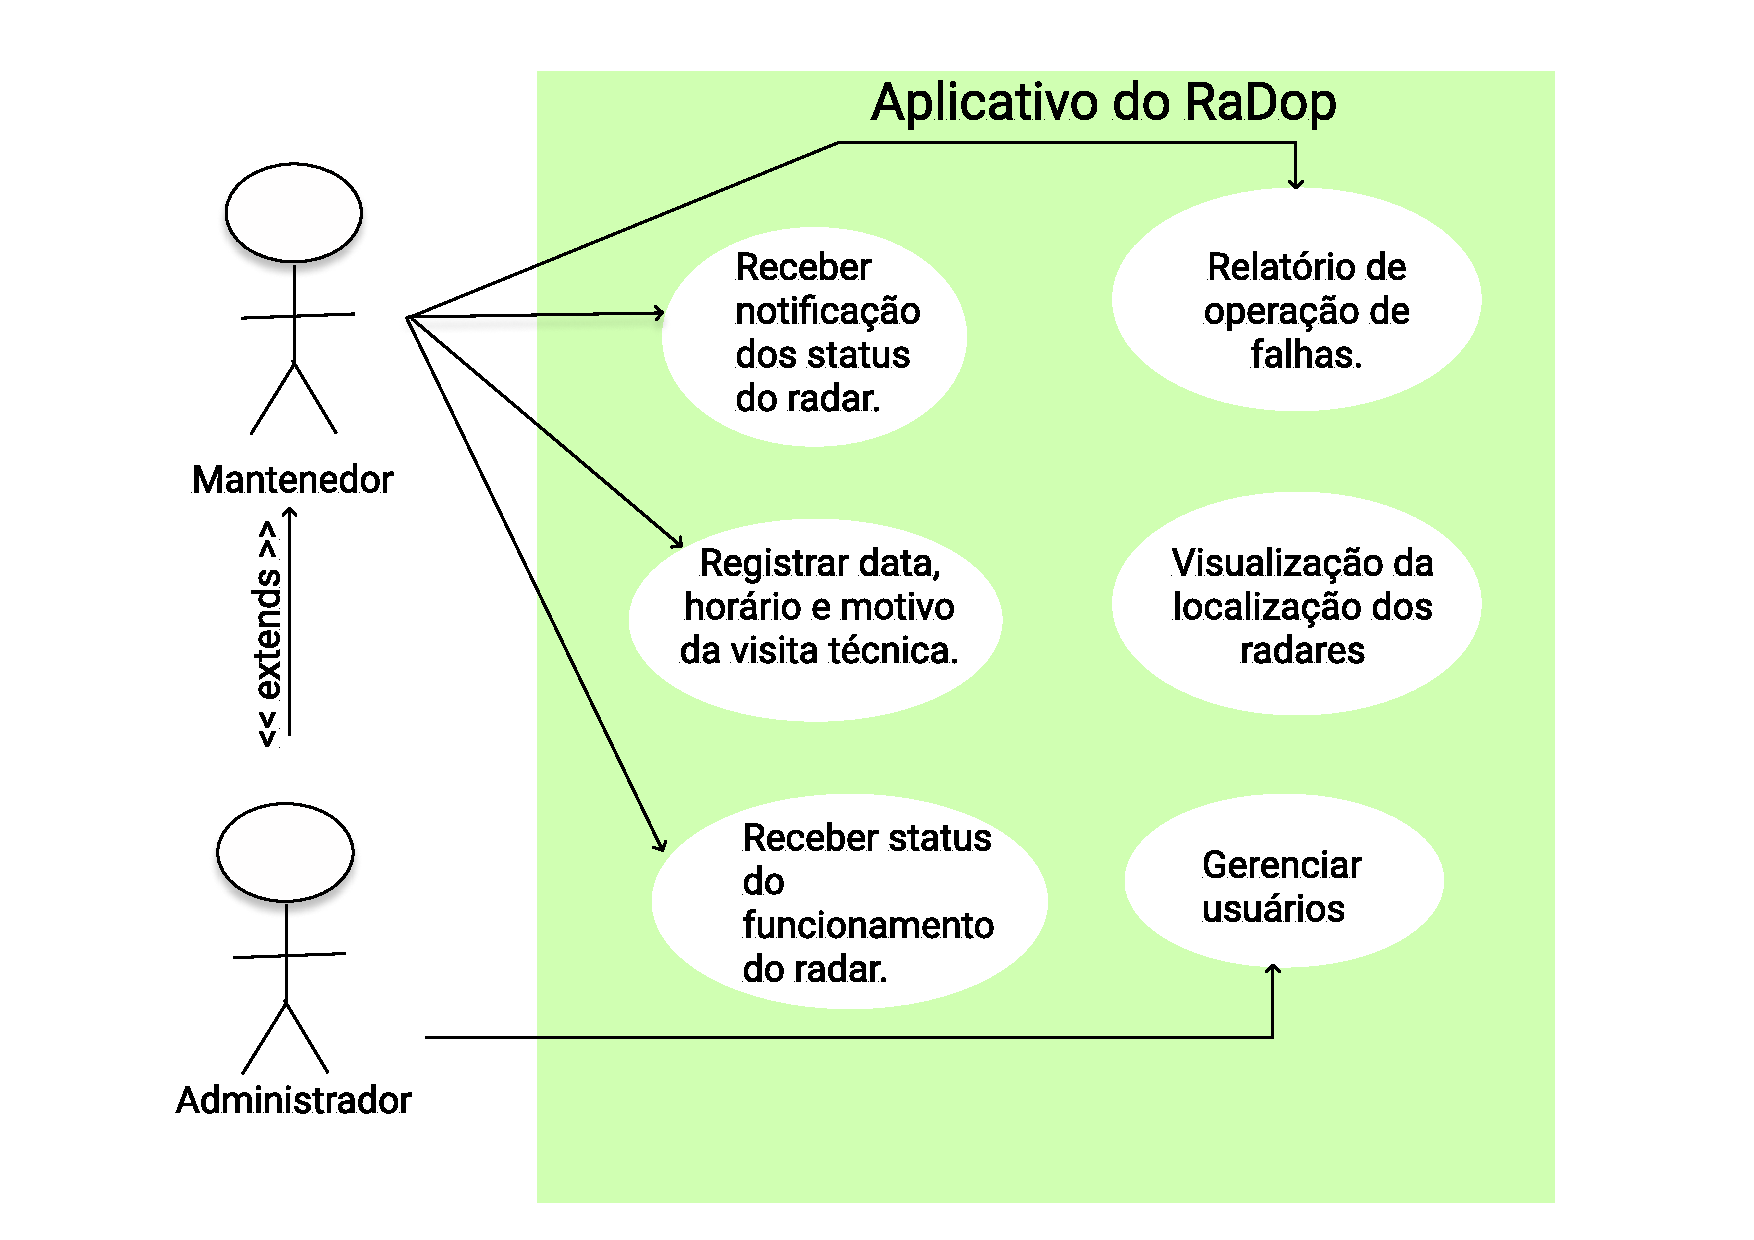
\includegraphics[scale=0.4]{caso_de_uso_2.pdf}}
	\caption{\label{fig:casos_de_uso} Diagrama de casos de uso com as principais funcionalidades do aplicativo RaDop.}
\end{figure}

A Figura \ref{fig:diagrama-comm-soft} apresenta o diagrama de casos de uso do \textit{Dashboard}.

\begin{figure}[H]
	\center{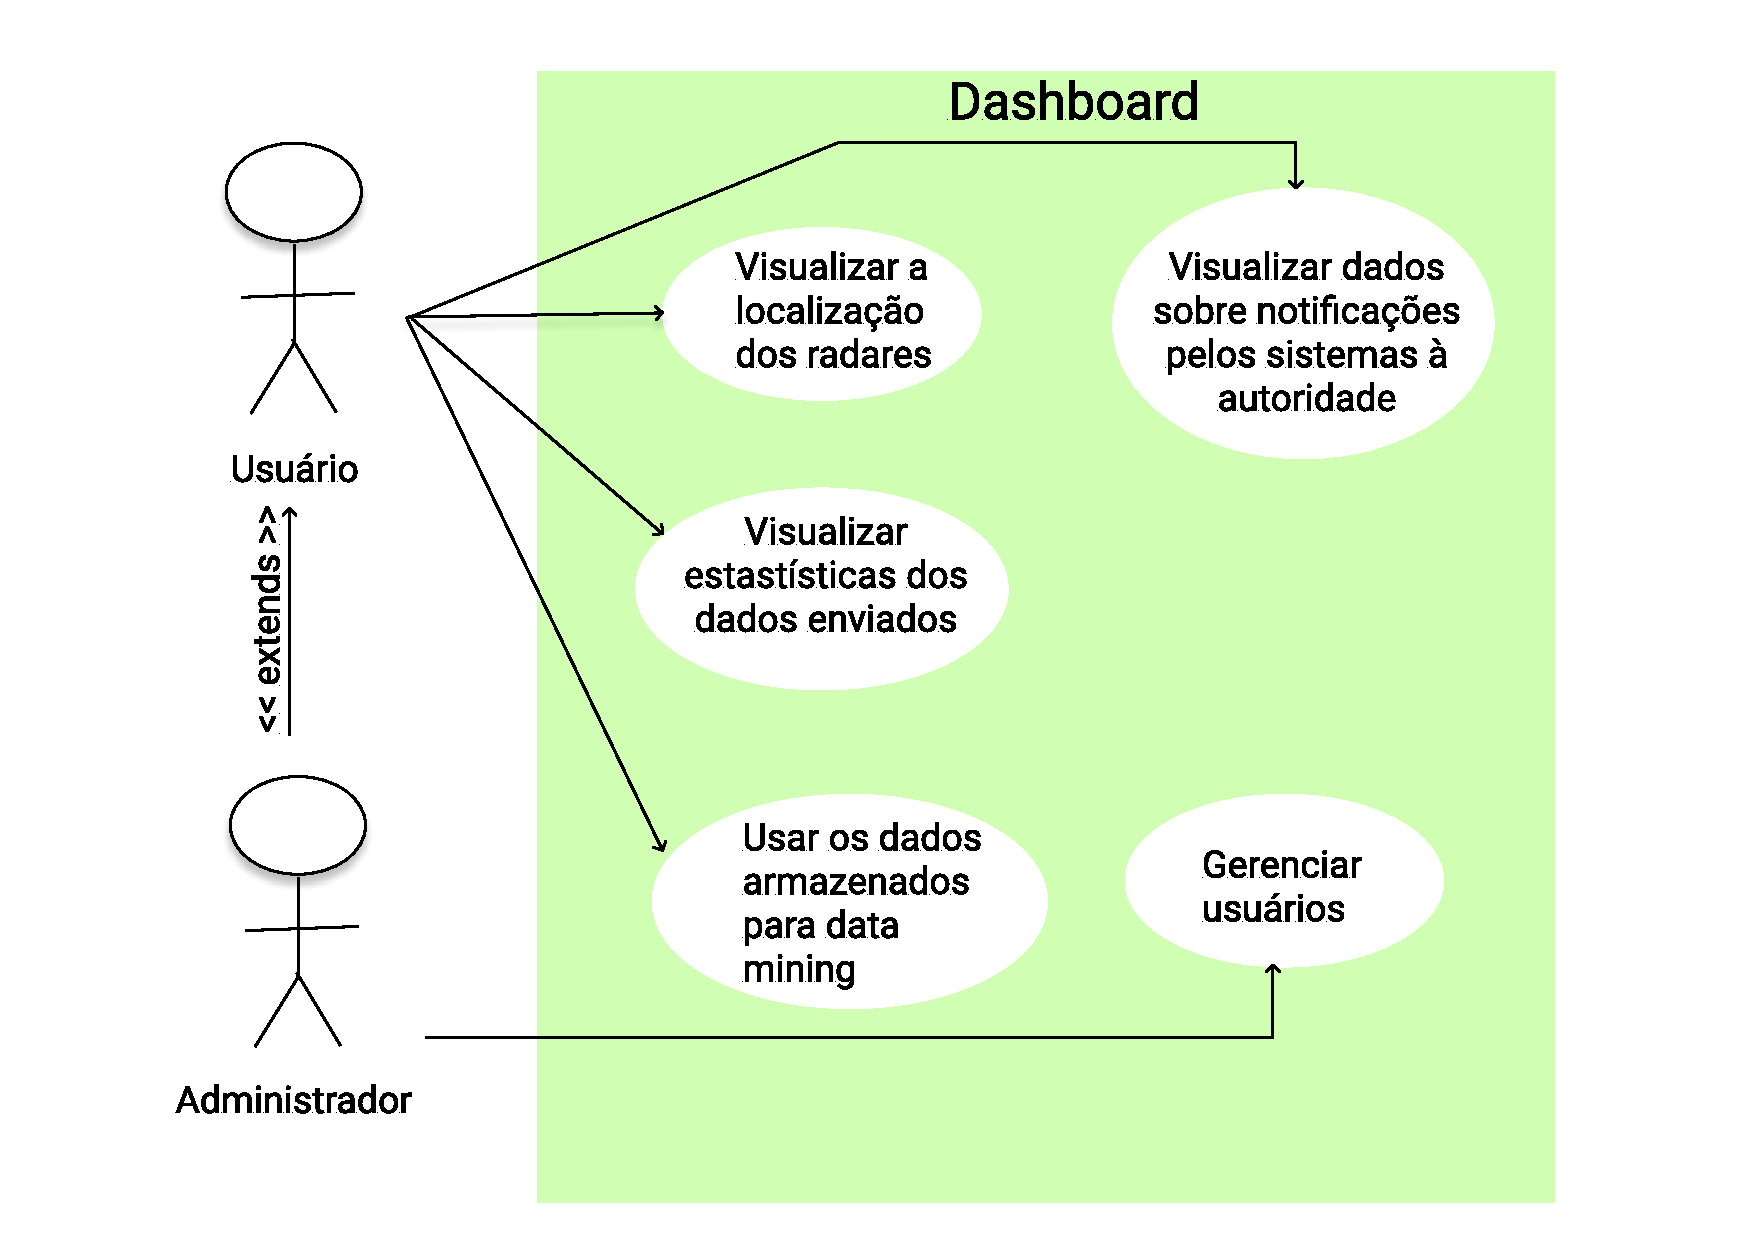
\includegraphics[scale=0.45]{caso_de_uso_1.pdf}}
	\caption{\label{fig:diagrama-comm-soft} Diagrama de casos de uso com as principais funcionalidades do \textit{Dashboard}.}
\end{figure}

\section{\textit{Dashboard}}

A arquitetura do \textit{Dashboard}, esquematizada na Figura \ref{fig:diagrama-arq-dashboard}, é principalmente baseada em componentes. O motivo para isso se deve ao uso do \textit{Django Application} do \textit{framework Django}, que é a principal tecnologia que é usada com o \textit{Dashboard}.

\begin{figure}[H]
	\center{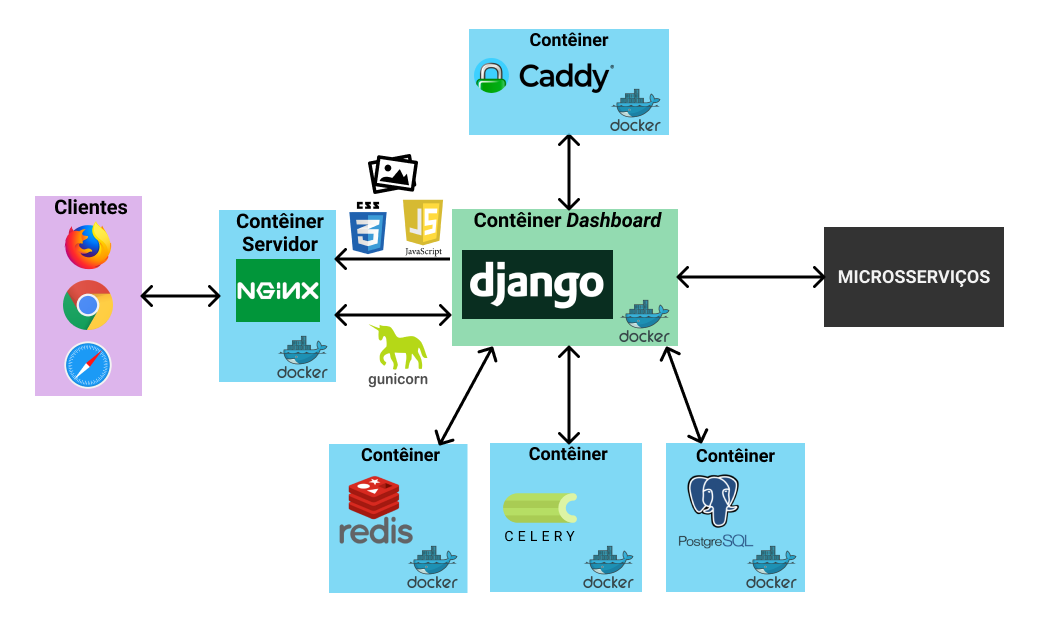
\includegraphics[scale=0.35]{diagrama-arq-dashboard.png}}
	\caption{\label{fig:diagrama-arq-dashboard} Diagrama que mostra a arquitetura e tecnologias que são usadas com o \textit{Dashboard}.}
\end{figure}

O uso de componentes permite uma série de vantagens. A primeira é construir componentes com alta coesão e baixo acoplamento, melhorando a manutenibi-lidade do código. Outra é que eles podem ser totalmente independentes entre si. As vantagens citadas acabam permitindo que componentes criados possam ser reaproveitados em vários projetos, evitando retrabalho desnecessário e assim otimizando o tempo dos desenvolvedores envolvidos no projeto.

Uma tecnologia importante que também é utilizada em conjunto com o \textit{Dashboard} é o NGINX. Ele é utilizado para fazer o \textit{proxy} reverso da aplicação. Explicando de modo resumido, ele atua como uma espécie de organizador, redirecionando as requisições que chegam dos clientes para os contêineres corretos.


\section{Aplicativo RaDop}

Conforme mostra a Figura \ref{fig:diagrama-arq-webApp}, o aplicativo móvel que auxilia a equipe de manutenção não acessa o radar diretamente, mas sim através dos microsserviços. Deste modo, os microsserviços funcionam como uma interface entre o radar e o aplicativo. Dessa forma é possível integrar mais facilmente todas as informações e compartilhá-las entre os produtos de software, mantendo os usários informados em todas as plataformas. 

O aplicativo foi construído em React-Native para \textit{smartphones Android} com versão superior a 5.0 (conforme elicitado na seção de requisitos). Neste formato pode ser construído versões da aplicação para \textit{smartphones Apple} que rodam o sistema \textit{iOS} sem a necessidade de construir uma nova versão.

\begin{figure}[H]
	\center{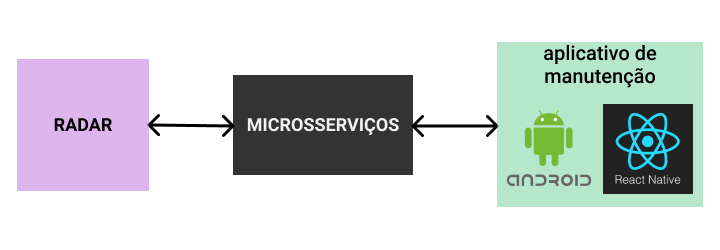
\includegraphics[width=\textwidth]{diagrama-arq-webApp.png}}
	\caption{\label{fig:diagrama-arq-webApp} Diagrama que mostra a arquitetura e tecnologias que são usadas com o \textit{WebApp}.}
\end{figure}

\subsection{Execução}

Após a fase de definição do projeto RaDop, a construção da aplicação foi iniciada conforme o esperado. Durante a construção surgiu a necessidade de criar um novo microsserviço de suporte para o aplicativo. Se trata de uma \textit{API Rest} para persistir os dados do funcionamento do \textit{app} e para auxiliar em outras funções, como o registro e autenticação de usuários. Esse serviço é melhor explicado na próxima seção deste documento. A seguir estão imagens tiradas do aplicativo em execução.

A Figura \ref{fig:app-sign-in} apresenta a tela construída para a autenticação dos usuários mantenedores dos radares.

\begin{figure}[H]
	\center{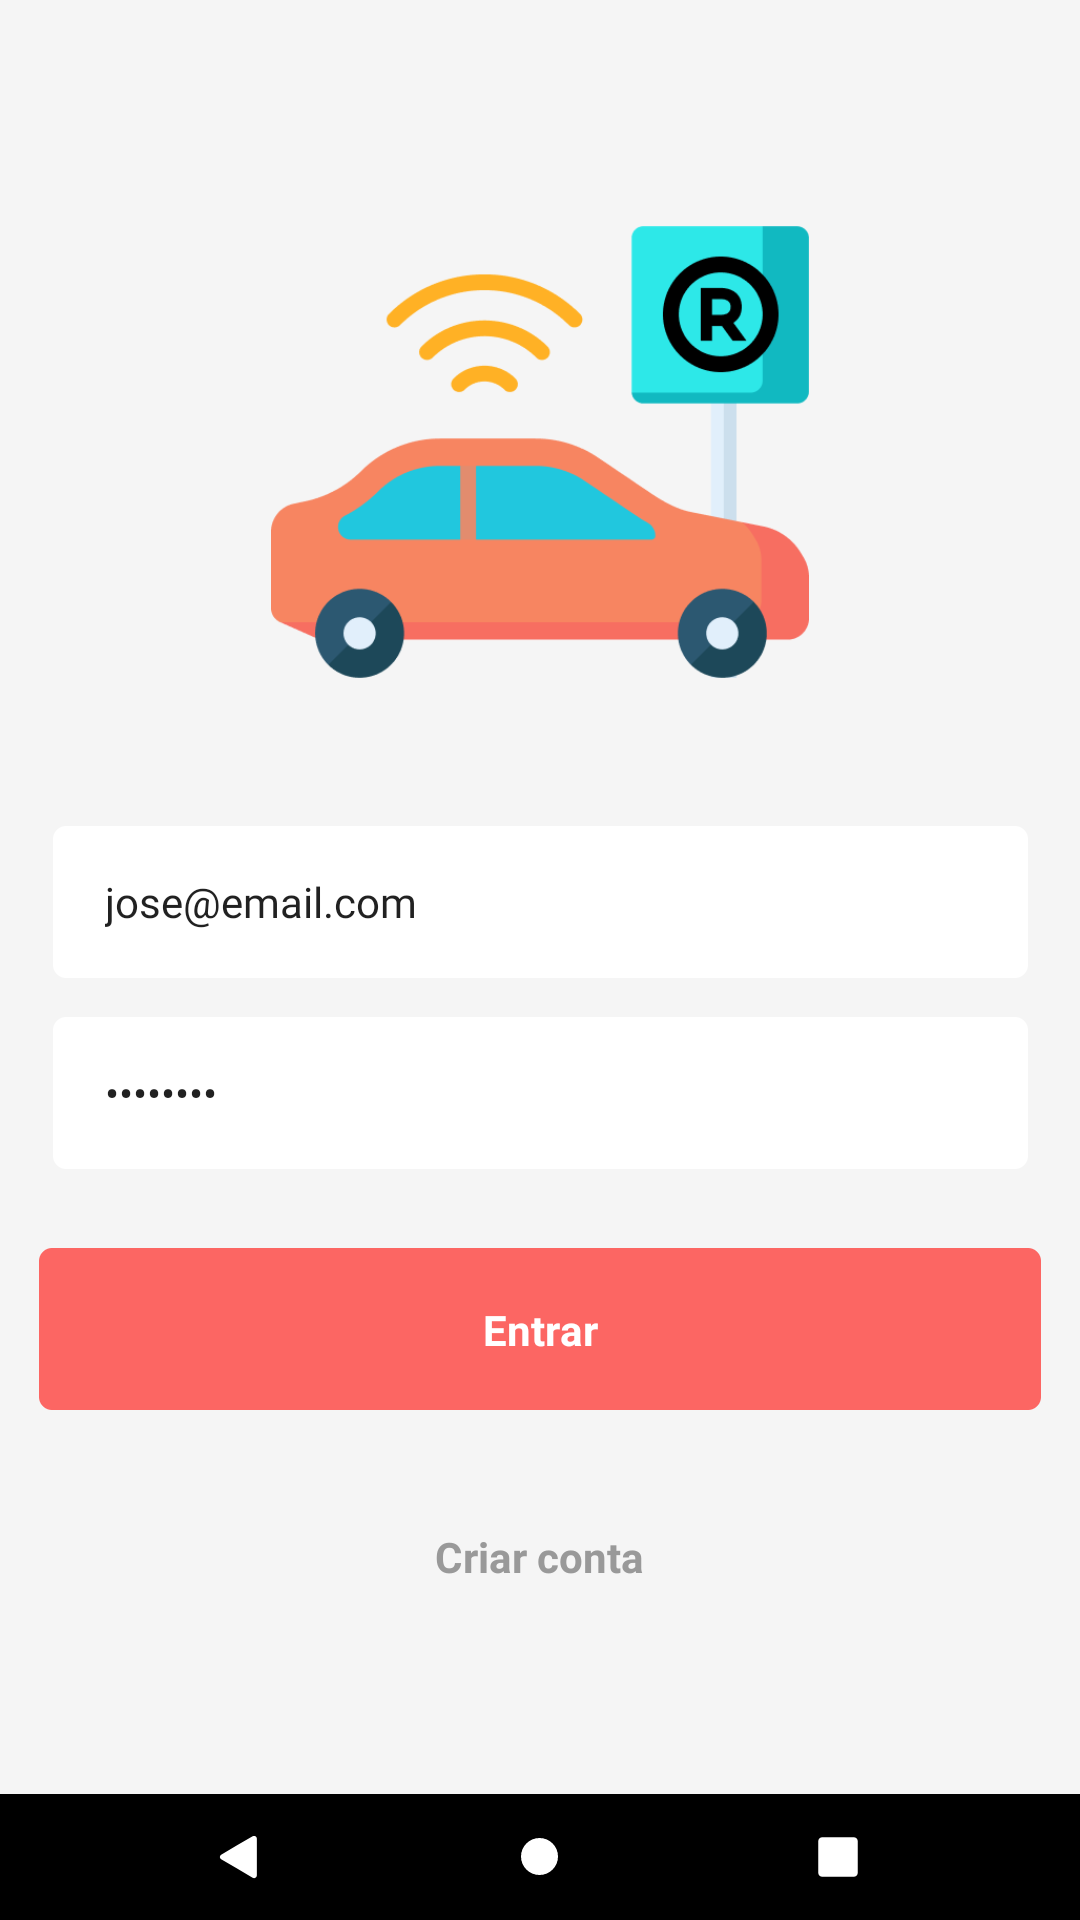
\includegraphics[scale=0.25]{login-final.png}}
	\caption{\label{fig:app-sign-in} Tela construída para a autenticação (\textit{login}) dos usuários.}
\end{figure}

A Figura \ref{fig:app-tela-principal} apresenta a tela inicial da aplicação. Nesta tela é possível identificar todos os radares num raio de 15Km a partir do ponto central GPS do dispositivo do usuário.

\begin{figure}[H]
	\center{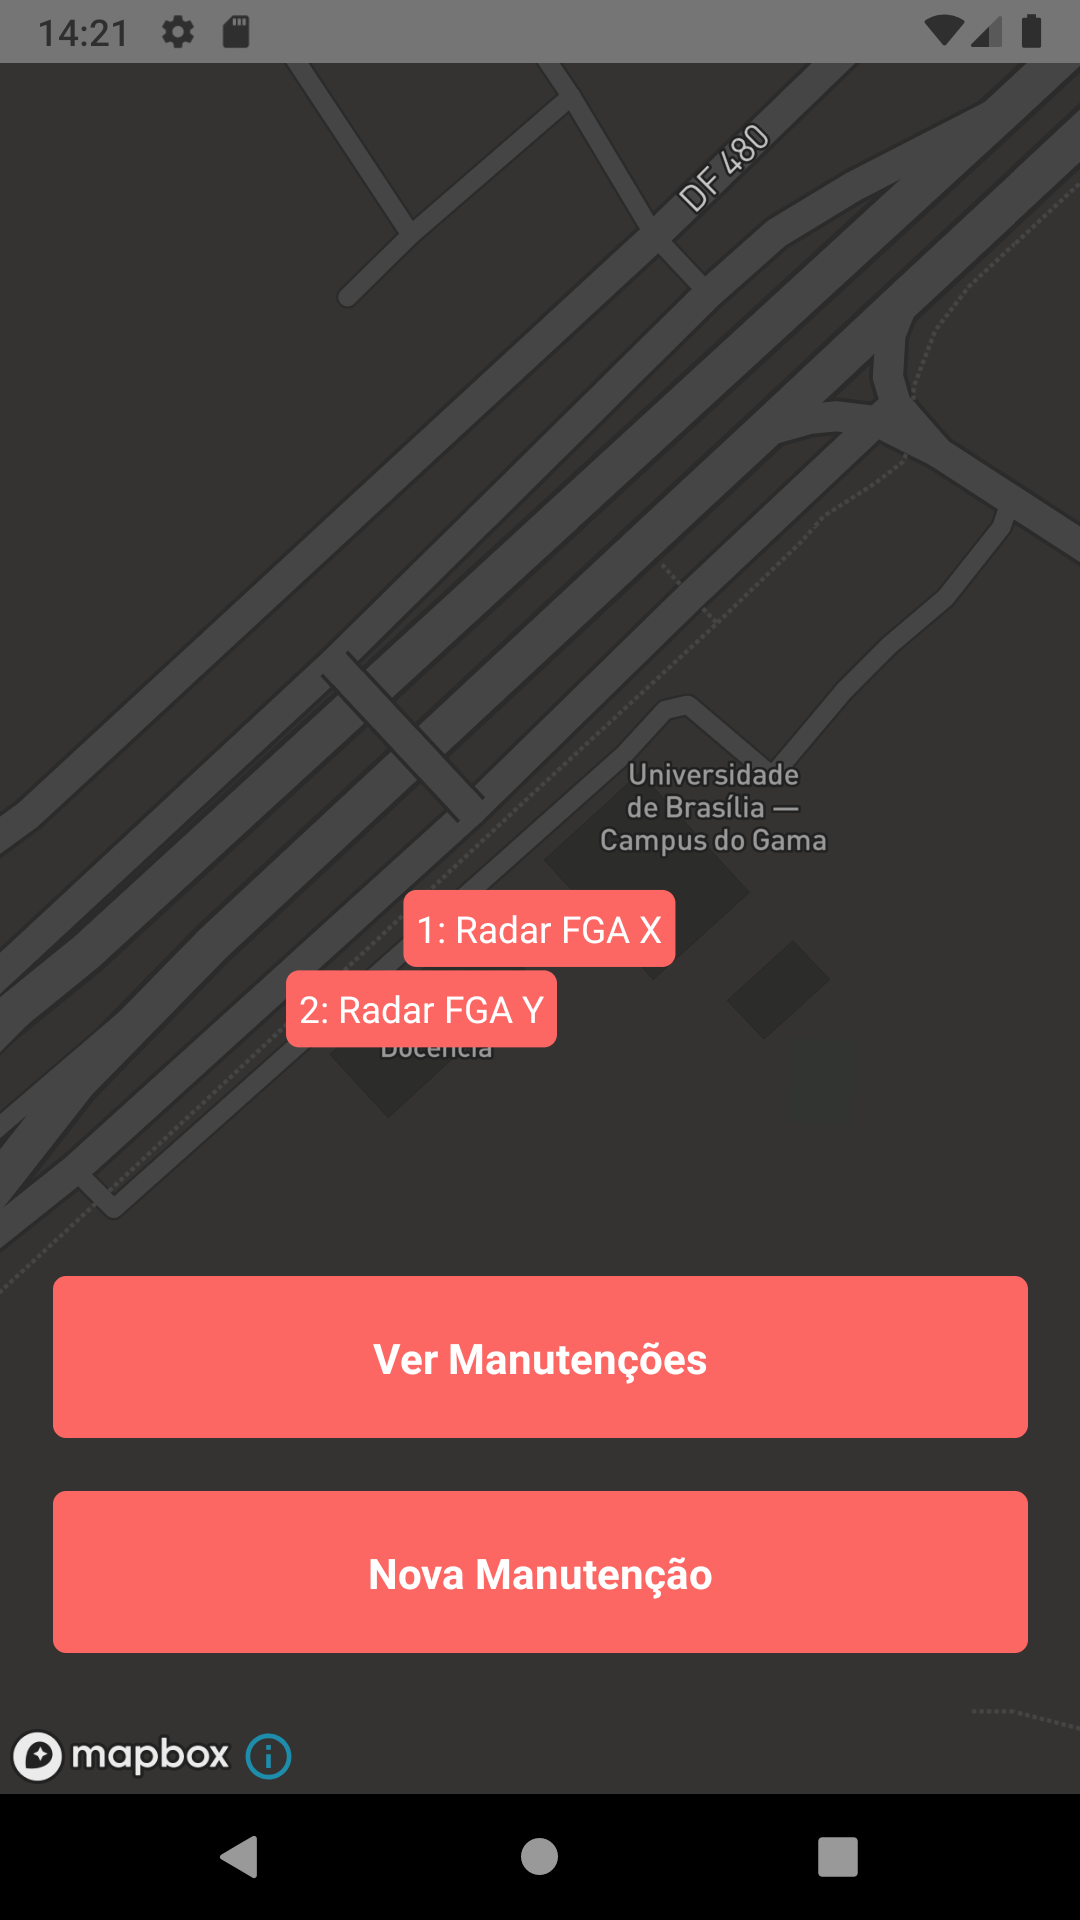
\includegraphics[scale=0.25]{inicial.png}}
	\caption{\label{fig:app-tela-principal} Tela construída para mostrar todos os radares próximos aos funcionários mantenedores (a partir do mapa no ponto central do dispositivo).}
\end{figure}

A Figura \ref{fig:status} apresenta a tela listando os últimos dez estados (\textit{status}) para o radar selecionado. Aqui é possível ver a indicação da operacionalidade do (da esquerda para direita):
\begin{itemize}
    \item Radar;
    \item Camêra;
    \item USRP;
    \item NFR.
\end{itemize}

\begin{figure}[H]
	\center{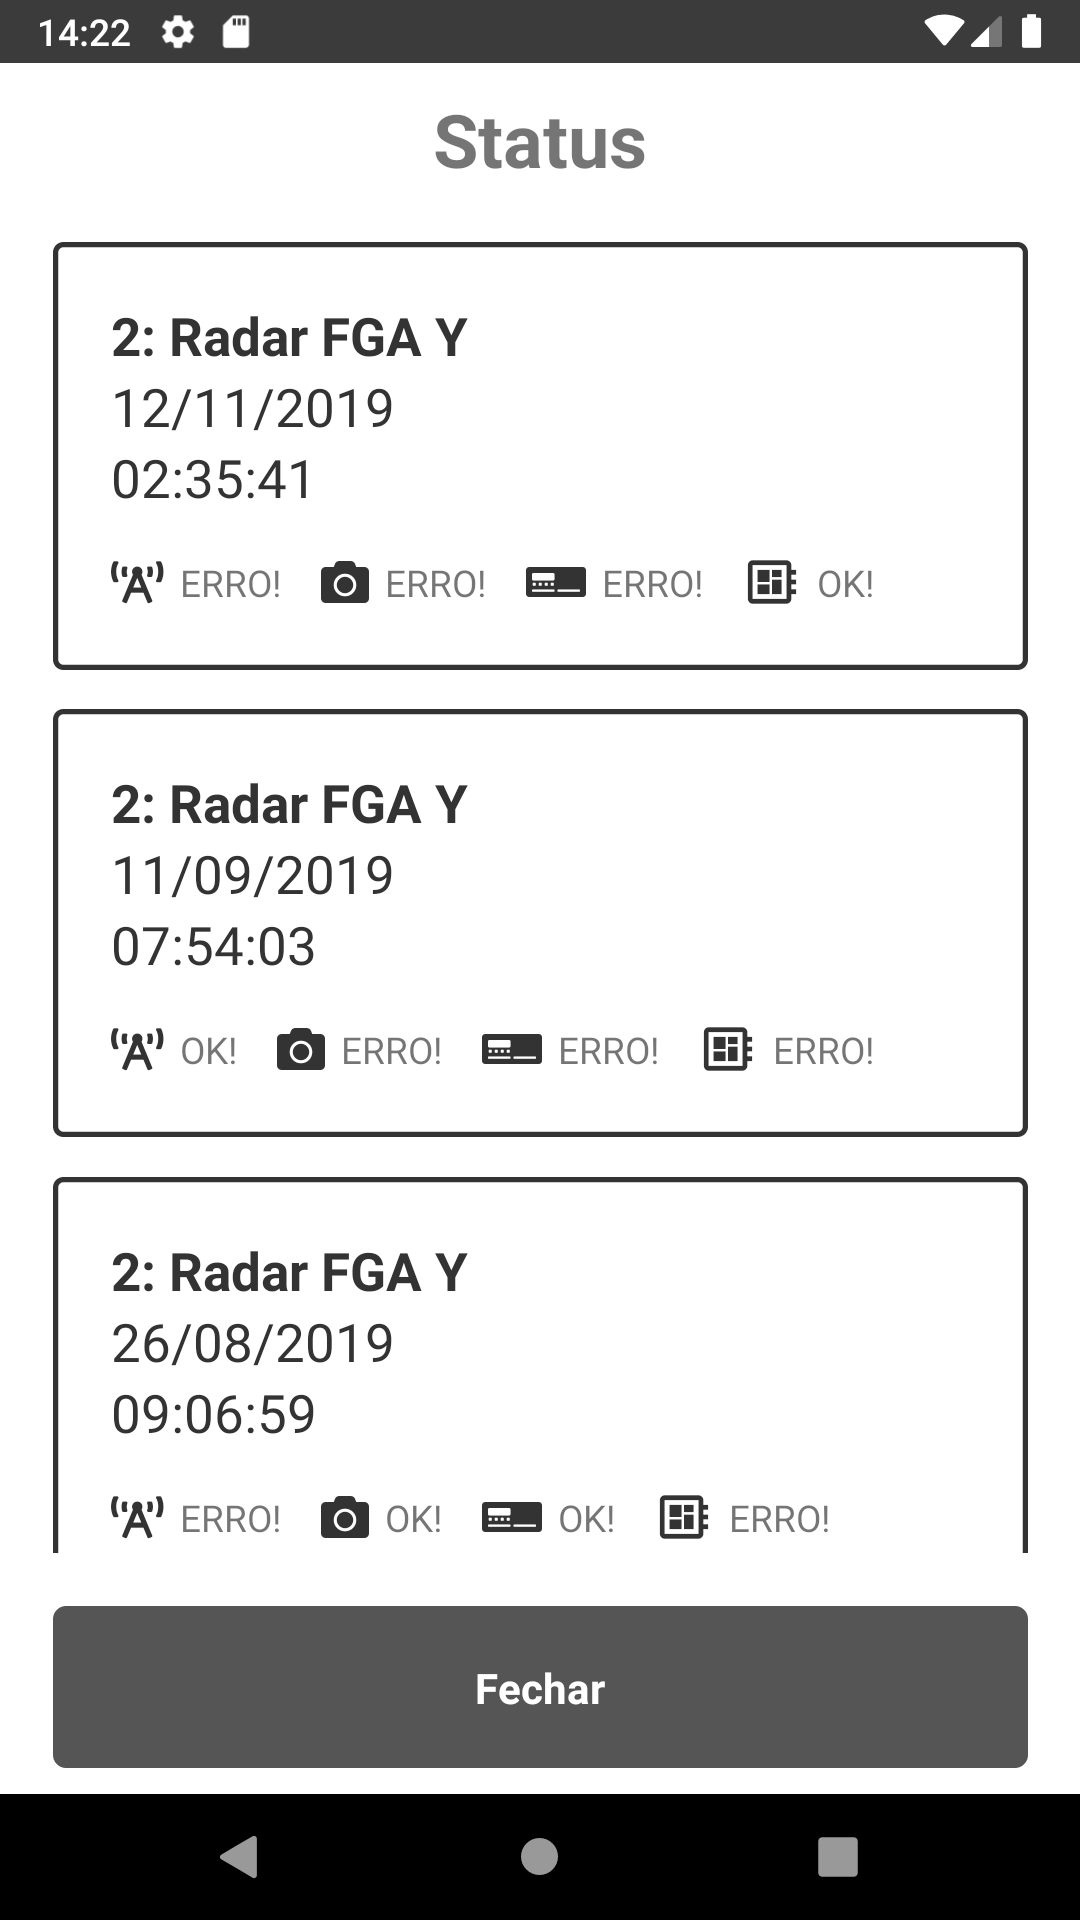
\includegraphics[scale=0.25]{status.png}}
	\caption{\label{fig:status} Tela com os estado de operação dos componentes do radar.}
\end{figure}

A Figura \ref{fig:manutencao-app} apresenta a tela de registro de uma nova manutenção para o radar selecionado no mapa.

\begin{figure}[H]
	\center{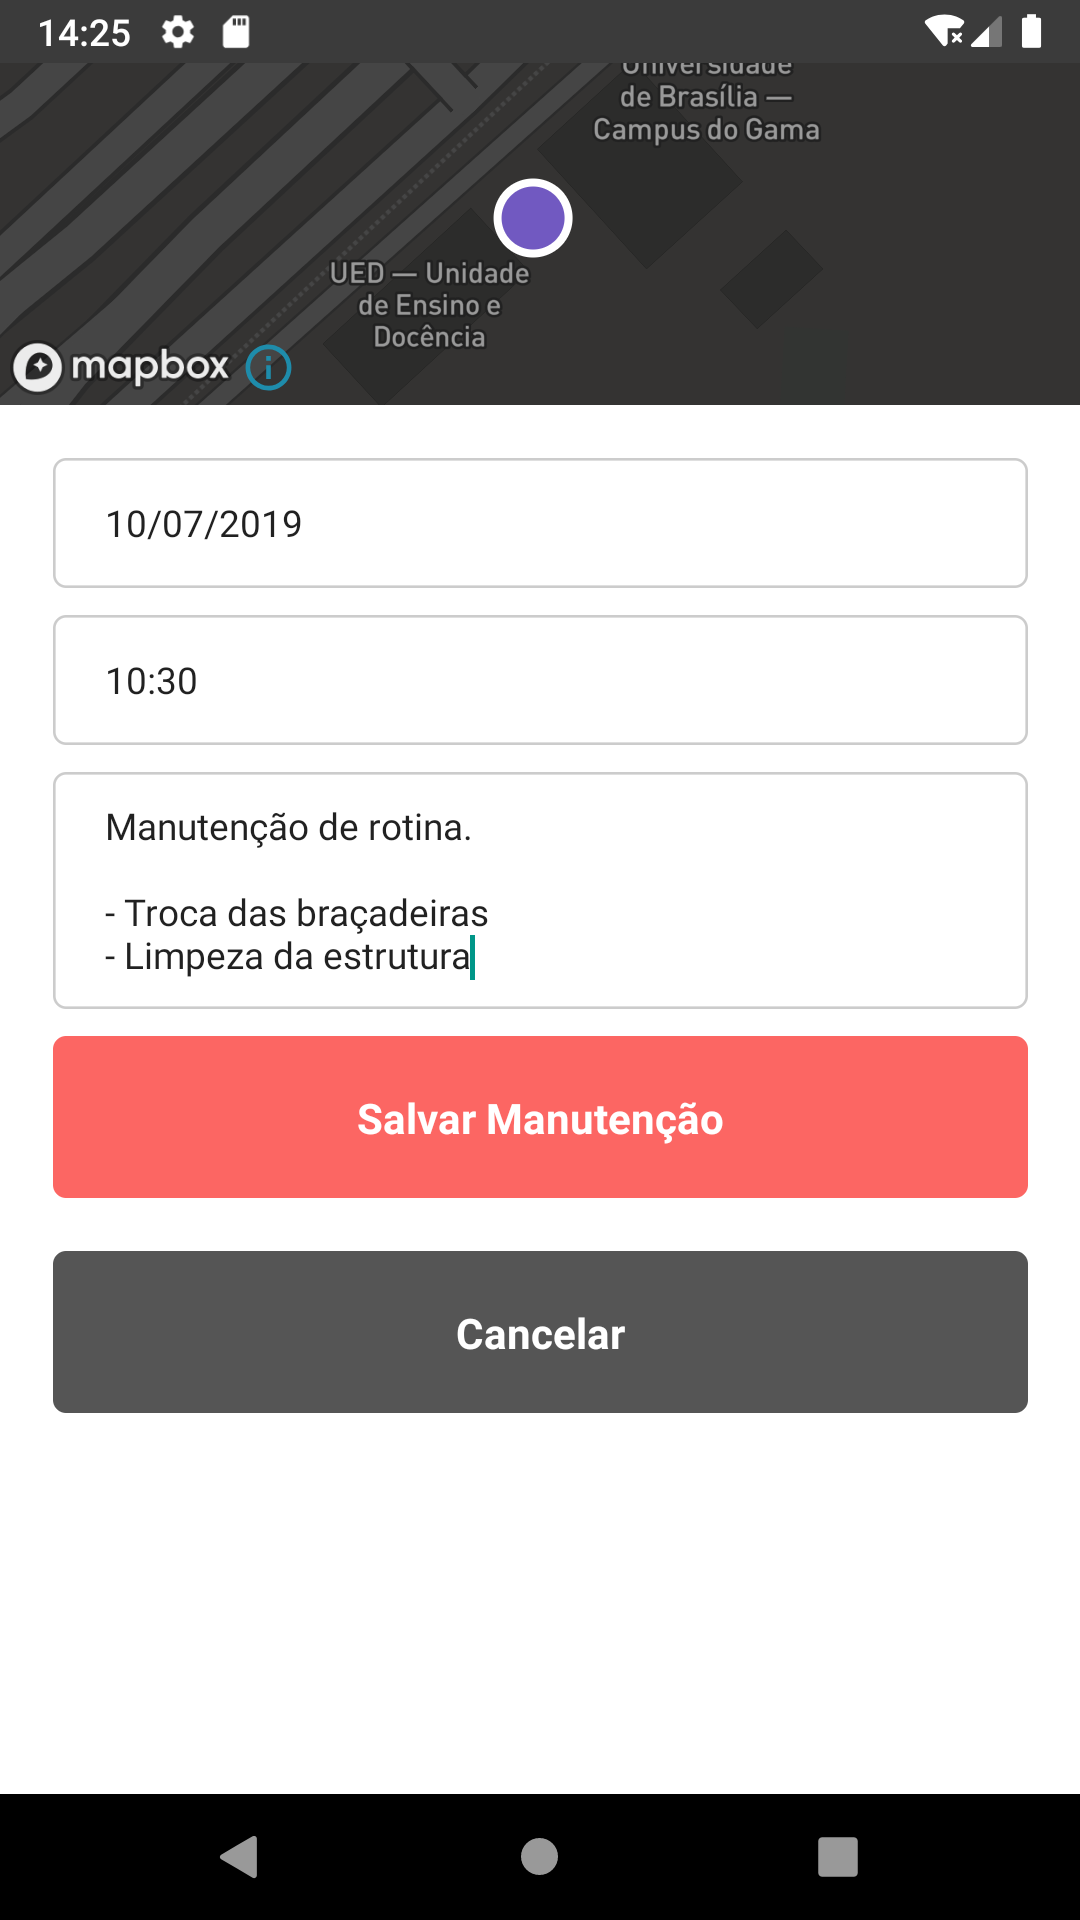
\includegraphics[scale=0.25]{manutencao.png}}
	\caption{\label{fig:manutencao-app} Tela com o formulário de manutenção do radar.}
\end{figure}


\section{Microsserviços}

Conforme definido na fase de iniciação de projeto do radar RaDop e anteriormente citado, além do aplicativo e do \textit{WebApp} de \textit{Dashboard}, alguns dos outros serviços de software são montados no formato de microsserviços, cuja arquitetura está esquematizada na Figura \ref{fig:diagrama-arq-microsservicos}.

\begin{figure}[H]
	\center{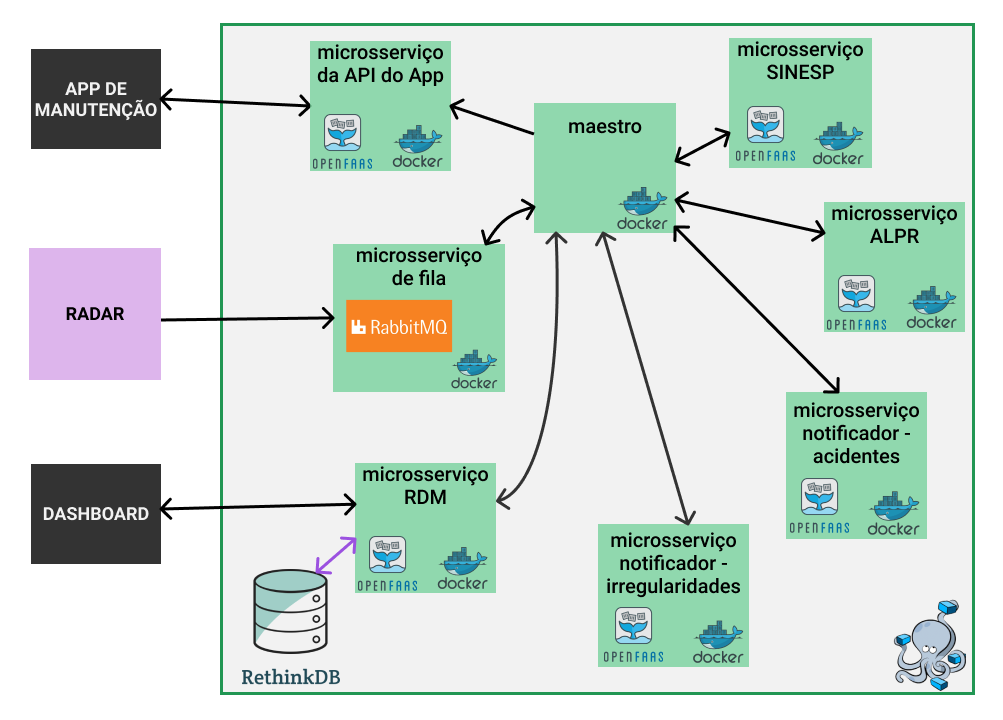
\includegraphics[width=\textwidth]{diagrama-arq-microsservicos.png}}
	\caption{\label{fig:diagrama-arq-microsservicos} Diagrama que mostra a arquitetura e tecnologias que são usadas com os microsserviços.}
\end{figure}

Logo, a partir da elicitação dos requisitos, tanto do projeto quanto dos outros produtos de software, a equipe levantou quais são os microsserviços que devem ser construídos. 

Lembrando que microsserviço é uma abordagem para desenvolver uma única aplicação como uma suíte de serviços, cada um rodando em seu próprio processo e se comunicando entre eles através de mecanismos leves. Segundo Fowler e Lewis \cite{fowler2015}, estes serviços são construídos através de pequenas responsabilidades e publicados em produção de maneira independente.

Alguns dos microsserviços são produzidos no formato de função como serviço (\textit{FaaS} - \textit{Function as a Service}). Segundo Freitas \cite{freitas2018}, essas funções são um serviço de computação em nuvem que busca abstrair a questão de servidor e máquinas onde rodam os seus programas. Em detalhes, ela deriva da filosofia \textit{Servless}, que delega ao provedor da computação em nuvem (\textit{Cloud Provider}) provisionar uma plataforma que permita ao cliente: desenvolver, rodar e gerenciar aplicações. Nestes moldes, reduz-se a complexidade de uma pessoa ter que montar e manter a infraestrutura, que é o atual padrão do mercado corporativo. Ao Montar uma aplicação com este padrão é implementada a teoria \textit{Servless} e criada uma arquitetura nativa de microsserviços.

Os microsserviços utilizados neste projeto são:

\begin{itemize}
    \item Microsserviço para a orquestração dos demais microsserviços (Maestro);
    \item Microsserviço para processar imagens de automóveis enviados radar (ALPR);
    \item Microsserviço para verificar a situação de veículos no banco de placas do SINESP;
    \item Microsserviço de banco de dados para armazenamentos de informações dos serviços (\textit{RethinkDB});
    \item Microsserviço de fila de mensagens (\textit{MQ - Message Queue});
    \item Microsserviço de servidor para o aplicativo RaDop (armazena as manutenções e informações relacionadas com a aplicação);
    \item Microsserviço de notificação de veículos flagrados excedendo a velocidade da via;
    \item Microsserviço de notificação de possíveis/prováveis acidentes.
\end{itemize}

Devido à filosofia dos microsserviços e às necessidades específicas de cada serviço, cada um é programado na linguagem e utilizando o \textit{framework} que me-lhor atenda à equipe e às expectativas do produto.

Caso haja necessidade de remoção, criação ou especialização dos serviços, a equipe de software faz as devidas alterações e comunica aos demais membros fora da equipe que possam ser afetados, assim como faz ou atualiza as documentações do projeto relevantes.

\subsection{Maestro}
Para o funcionamento bem sucedido dos microsserviços do projeto, eles têm que interagir entre si e também com sistemas externos -- radar, \textit{Dashboard} e \textit{WebApp}. Mas a maneira como se dá essa relação varia de acordo com a situação. Como a base dos microsserviços é mantê-los granulares e o mais independentes possível, é usado no projeto um orquestrador, chamado Maestro.

\subsubsection{Uso no RaDop}
A função do orquestrador é articular os diversos subsistemas e o radar, de modo a alcançar um determinado objetivo. Esse objetivo é determinado pela mensagem que for recebida pelo Maestro, que é o ponto de partida para ele começar a orquestrar o trabalho. Por isso, ele tem conhecimento de todos os microsserviços e sistemas externos, pois se comunica com eles para completar suas tarefas.

\subsubsection{Execução}
Para o correto funcionamento do Maestro, foi necessário primeiro fazer com que ele se comunique com o RabbitMQ. Isso porque as mensagens, que carregam as ordens de trabalho e dados para o orquestrador, chega através desse gerenciador de mensagens.

Recebida a mensagem, o orquestrador aciona os microsserviços necessários para cumprirem a tarefa. Quais e em que momento eles são acionados vai depender de qual foi a mensagem recebida inicialmente. Caso algum dado deva ser passado entre microsserviços ou entre esses e sistemas externos, é o orquestrador que o faz.

\subsection{ALPR}

ALPR são tecnologias que utilizam o OCR (\textit{Optical Character Recognition} ou reconhecimento óptico de caracteres) em imagens para reconhecer placas de veículos automotores regulados. A sigla ALPR significa \textit{Automated License Plate Recognition}, que são sistemas que a partir da leitura de caracteres reconhecem placas de veículos automotores.

\subsubsection{Uso no RaDop}

Dentro do projeto do radar RaDop, a equipe levantou a necessidade de fazer uso de tecnologias de reconhecimento de placas para informar às autoridades competentes sobre veículos infratores registrados pelo radar.

Com isso, imagens dos veículos infratores são capturadas por uma câmera conectada ao radar. Em seguida, são enviadas para o processamento e reconhecimento por um serviço que é construído pela equipe de software do projeto.

A equipe de software, após analisar ferramentas de OCR e ALPR optou por usar o \textit{OpenALPR}, devido à completude da ferramenta e à restrições financeiras -- o \textit{OpenALPR} apresenta um subproduto gratuito que atende às necessidades da equipe.

Outros fatores relevantes para a decisão do uso do \textit{OpenALPR} foram o tempo curto disponível e as dificuldades caso fosse feito o treinamento de uma máquina em OCR para realizar o ALPR dentro do prazo disponível. Se a equipe optasse por realizar esse treinamento, o custo do projeto aumentaria consideravelmente e possivelmente teriam atrasos no cronograma, correndo-se o risco até do aprendizado da máquina não ser completamente executado. Os principais complicadores são:

\begin{itemize}
    \item Necessidade de ter muitas imagens de placas automobilísticas usadas no Brasil para que seja obtido um bom modelo a partir do treinamento;
    \item Tempo necessário para realizar treinamentos e reajustes no algoritmo usado -- e, dependendo do caso, até mudança de algoritmo -- para que seja obtido um modelo confiável (ou seja, com muitos acertos e boa generalização para imagens que não tenham sido usadas no aprendizado) para ser utilizado com as fotos que são enviadas pelos radares;
    \item Requerimentos de hardware (em especial placa de vídeo, memória RAM e processador) para o treinamento da máquina e no reconhecimento das placas. No presente momento, a equipe não possui esse equipamento à disposição e a compra dele encareceria bastante o orçamento do projeto.
\end{itemize}

O sistema é integrado ao servidor de serviços do RaDop por meio de uma API que se comunica com o \textit{OpenALPR} e é tratada dentro dos demais serviços de apoio do RaDop.

\subsubsection{Execução}

Para sanar a necessidade de identificação das placas, foi construído o serviço \textit{Fn-ALPR}. A \textit{Fn-ALPR} é a função responsável por tratar as imagens recebidas do radar e enviar à API do \textit{ALPR} para que seja feito o reconhecimento (OCR) dos caracteres da placa. Logo, com o dado enviado para este serviço é retornado um relatório com as placas encontradas na imagem. Portanto o serviço foi criado e integrado aos demais serviços para satisfazer as necessidades do radar.


\subsubsection{Testes}

Para validação da função criada para reconhecer as placas dos veículos, foram feitos testes com uso de imagens feitas pela camêra usada no radar. Na Figura \ref{fig:teste-alpr-foto-carro} está presente a imagem de um dos testes, assim como a representação do resultado obtido quando invocada a função \textit{Fn-ALPR}.

\begin{figure}[H]
	\center{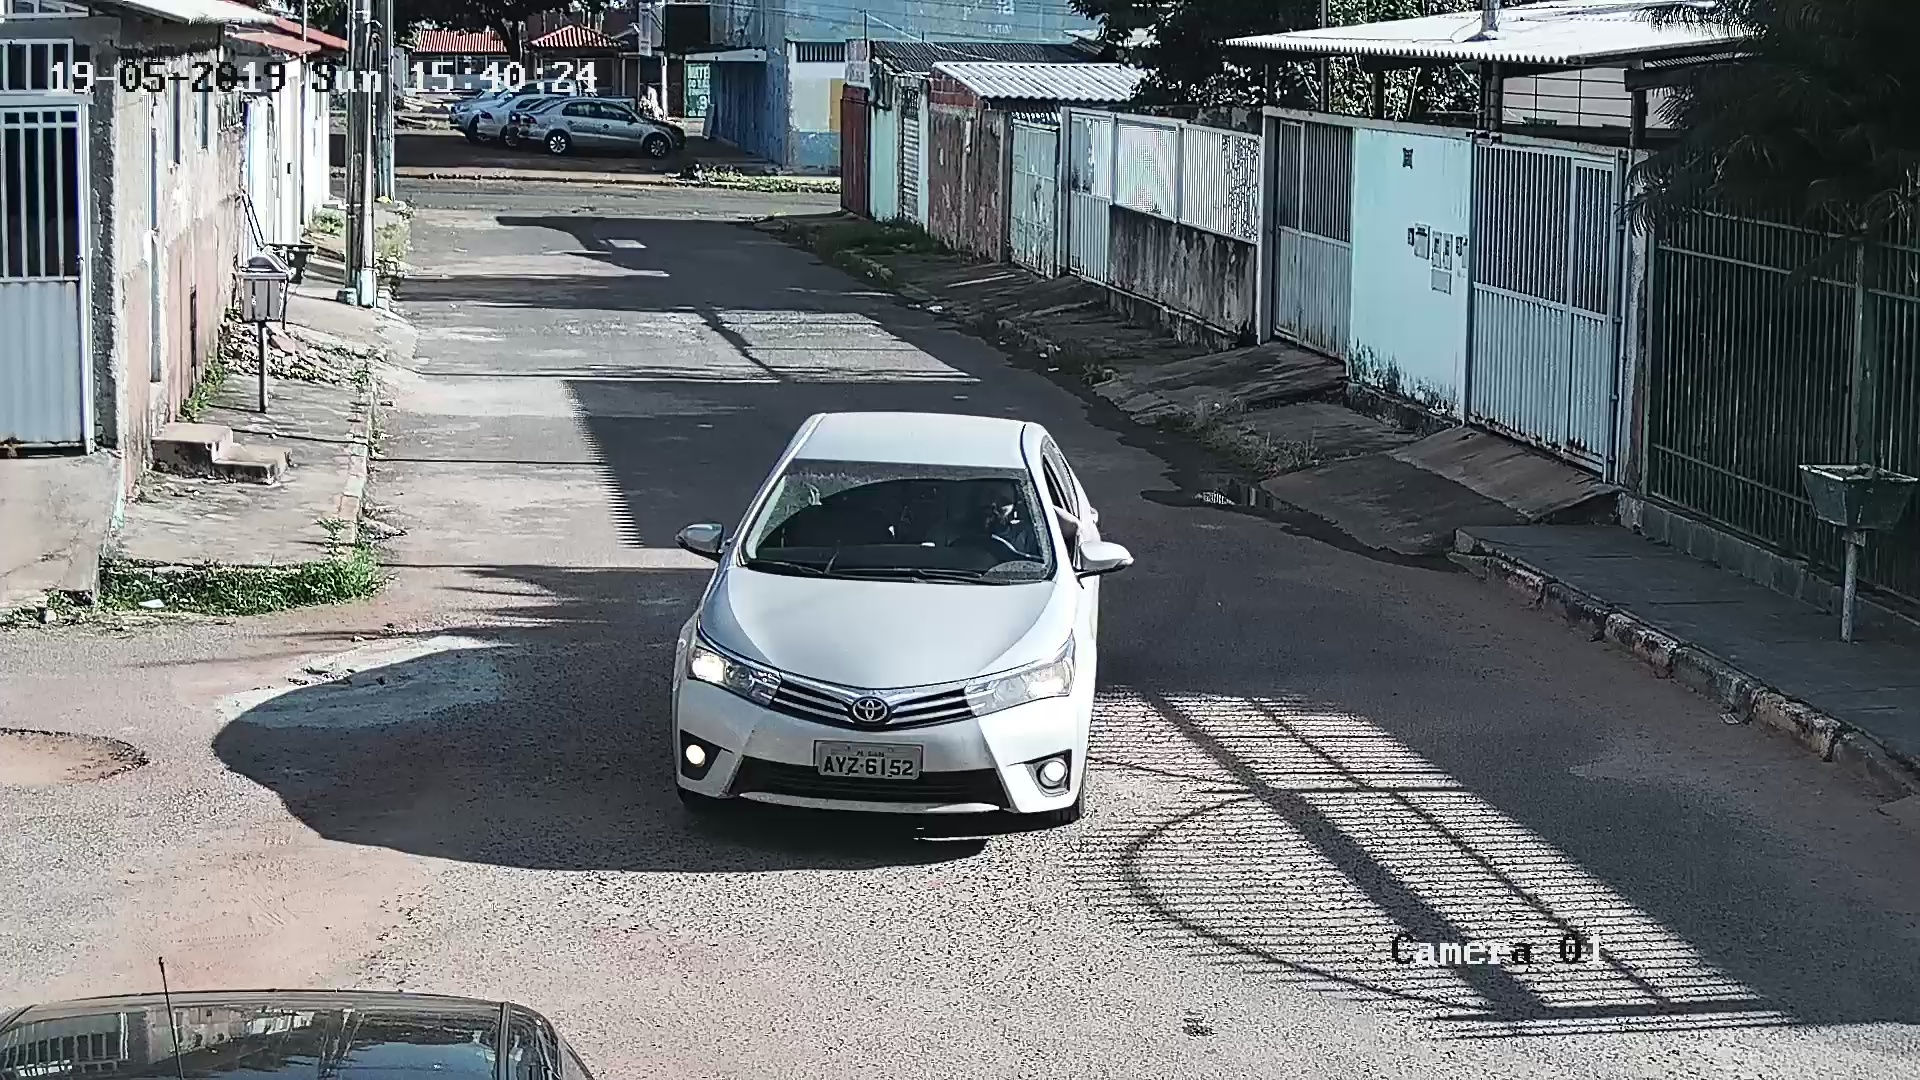
\includegraphics[scale=0.21]{teste-alpr.jpg}}
	\caption{\label{fig:teste-alpr-foto-carro} Imagem tirada com a camêra do radar e que foi enviada ao serviço para reconhecimento da placa.}
\end{figure}

No apêndice \ref{teste_alpr} está o código de resposta do servidor após a execução da \textit{Fn-ALPR}, com os resultados que foram capturados a partir da imagem. Dentro da chave \textit{results} há o objeto JSON com o melhor resultado da análise da imagem. Caso necessário, abaixo, existe a chave \textit{candidates}, que são outros prováveis resultados para a placa do carro.

\subsection{SINESP}

Após a execução do processamento de imagem através do \textit{ALPR}, é preciso obter informações do veículo flagrado. Para obter essas informações é preciso se comunicar com o SINESP.

Dentro do projeto do Radar, a equipe percebeu a necessidade de haver comunicação com o banco de dados do SINESP. Por isso, inicialmente foi criada a Função SINESP, ou Fn-SINESP, que era responsável por levantar dados sobre a situação de cada veículo no banco de dados da plataforma. De acordo com o modelo de dados enviado, o serviço pesquisava junto ao SINESP informação cadastrais, assim como situação, restrições, ano, modelo, cor e outras informações sobre o veículo informado.

Porém, devido à uma mudança de segurança da API do Sinesp, não foi possível continuar a utilização da Fn-SINESP. Após buscar por novas alternativas para o acesso ao SINESP, foi decidido utilizar um novo serviço, disponibilizado online. Através dele, apenas fornecendo a placa do veículo, é possível obter os mesmos dados que a Função disponibilizava.

\subsubsection{Teste}

Foram efetuados diversos testes de comunicação do microsserviço SINESP. A Figura \ref{fig:sinesp} tem um registro de como é feita a busca no banco de dados do SINESP e as informações retornadas por ele.

\begin{figure}[H]
	\center{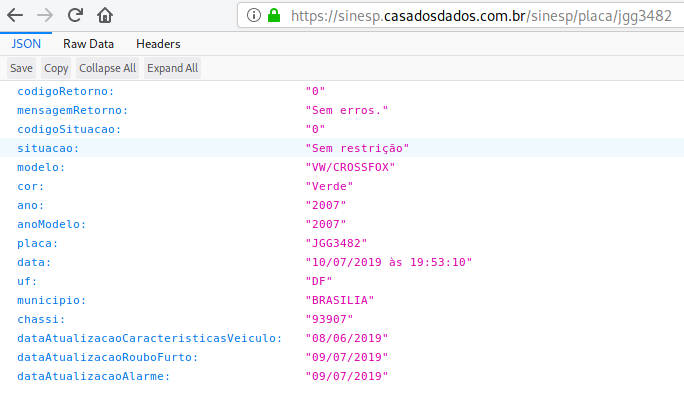
\includegraphics[width=\textwidth]{fn-sinesp.png}}
	\caption{\label{fig:sinesp} Resultado encontrado pelo ao pesquisar a placa JGG-3482 junto ao SINESP.}
\end{figure}

\subsection{\textit{Rethink Data Manager}}

O microsserviço \textit{Rethink Data Manager}, ou RDM,  é o serviço responsável por comunicar todos os sistemas com o banco de dados \textit{RethinkDB} do projeto (banco de dados NoSQL), além de suprir, via \textit{websocket}, um servidor para todas as operações do banco de dados.

Com isso, o RDM supre os demais sistemas com todas as operações comuns de um banco de dados -- as quais a equipe julgou necessário estarem presentes no sistema -- para que fosse possível persistir os dados dos microsserviços. 

A tecnologia \textit{websocket} é um protocolo que permite a comunicação bidirecional entre um cliente e um servidor. O modelo trabalha com um soquete TCP e foi inicialmente projetado para ser executado em navegadores web. O objetivo dessa tecnologia é fornecer um mecanismo para aplicações que precisam de comunicações bidirecionais com servidores que não dependam da abertura de várias conexões HTTP. O RDM utiliza desse formato de comunicação para receber e enviar dados que ele gerencia do banco de dados.

A Figura \ref{fig:rdm-server} mostra os \textit{logs} de execução do servidor do RDM. 

\begin{figure}[H]
	\center{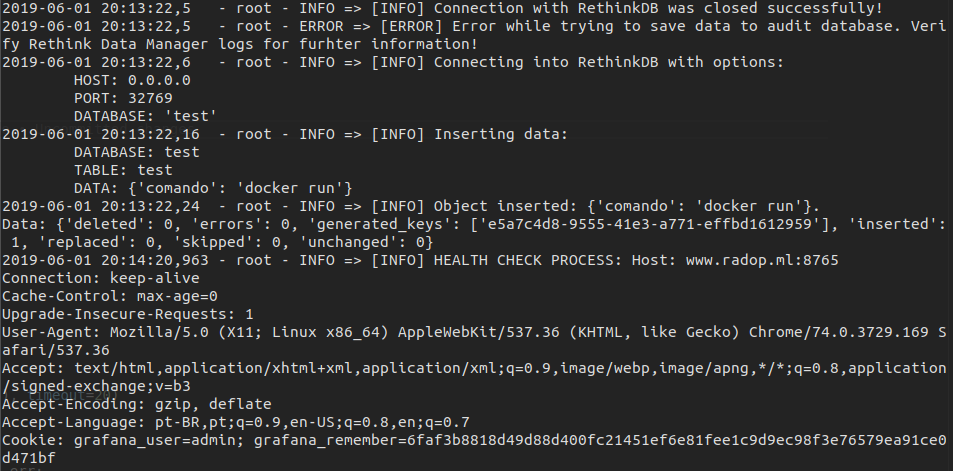
\includegraphics[scale=0.4]{rethink-manager-server.png}}
	\caption{\label{fig:rdm-server} Terminal com \textit{logs} de execução do servidor do RDM.}
\end{figure}

A Figura \ref{fig:rdm-cliente} mostra os \textit{logs} de execução de um cliente executando comandos no RDM. 

\begin{figure}[H]
	\center{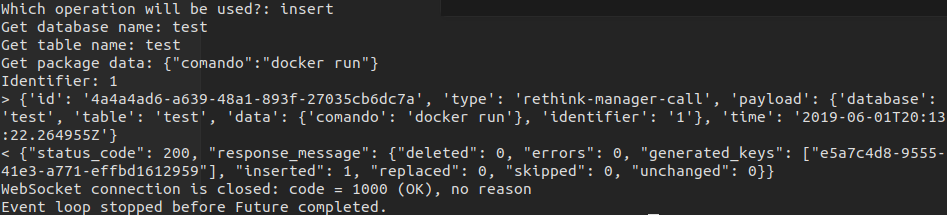
\includegraphics[scale=0.4]{rethink-manager-client.png}}
	\caption{\label{fig:rdm-cliente} Terminal com \textit{logs} de execução de um cliente executando comandos no RDM.}
\end{figure}

\subsection{RaDop App \textit{Server}}

O RaDop App \textit{Server}, ou RAS, é o serviço responsável pelo \textit{back-end} do aplicativo RaDop. Nesse serviço está contemplado os \textbf{CRUDs} (\textit{Create}, \textit{Read}, \textit{Update} e \textit{Delete}) necessário para o funcionamento do RaDop App, assim como as funções de autenticação de usuário.

Com isso, o RAS dá o suporte necessário para a persistência de dados da aplicação do RaDop, além de fornecer um serviço de autenticação seguro. Isso permite que o app seja mais completo e atenda todas as necessidades levantadas pela equipe do projeto. Para verificar as rotas e o funcionamento da API verifique no link do \textit{Swagger} todas as operações disponíveis para este serviço -- \href{https://app.swaggerhub.com/apis-docs/sconetto/RaDop_App_Server/1.0.0-ALPHA}{RAS API Swagger Docs}.

A Figura \ref{fig:radop-app-server} apresenta a execução do serviço dentro do servidor RaDop por meio de \textit{logs} de funcionamento.

\begin{figure}[H]
	\center{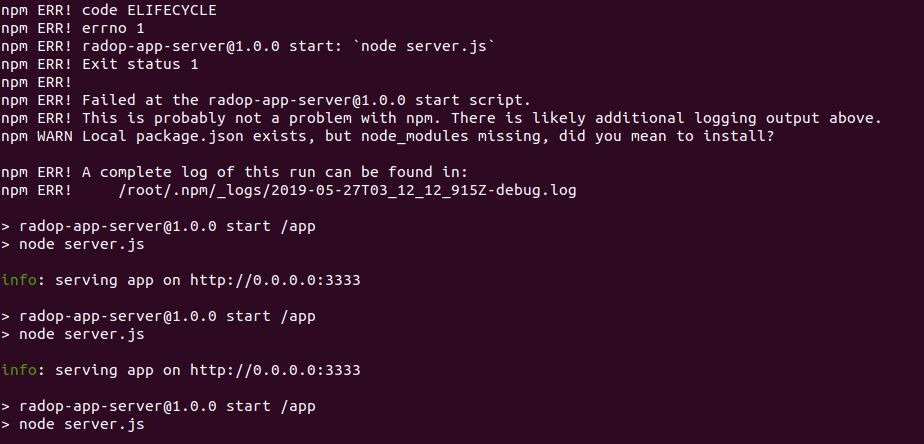
\includegraphics[scale=0.4]{radop-app-server.png}}
	\caption{\label{fig:radop-app-server} \textit{Logs} de execução do RaDop App \textit{Server} indicando a sua disponibilidade.}
\end{figure}

\subsection{Protocolo de Comunicação de Software}

O \textit{stack} de produtos de software que são produzidos devem, em certos momentos da execução, comunicarem-se internamente. Para a correta execução, a equipe de software previu interfaces para a comunicação dos produtos de software, algumas que posteriormente são utilizadas também para a integração com a equipe de eletrônica.
Os tipos de interfaces para a comunicação dos serviços são:
\begin{itemize}
    \item \textbf{HTTP}:
    A sigla para \textit{Hypertext Transfer Protocol}, se trata de um protocolo de comunicação (na camada de aplicação segundo o Modelo OSI) de transferência de hipertexto utilizado para sistemas de informação de hipermídia, distribuídos e colaborativos.
    \begin{enumerate}
        \item \textbf{Aplicativo RaDop}: Se comunica com a nuvem de serviços a partir do HTTP, usando ele para fazer requisições de serviços;
        \item \textbf{\textit{WebApp Dashboard}}: Se comunica com os serviços no mesmo formato do aplicativo, através de requisições com envio de pacotes HTTP.
    \end{enumerate}

    \item \textbf{HTTPS}:
    Uma evolução do HTTP, o \textit{Hypertext Transfer Protocol Secure}, ou HTTPS, é uma implementação do HTTP sobre uma camada adicional de segurança que utiliza o protocolo SSL/TLS.
    \begin{enumerate}
        \item \textbf{Banco de Dados NoSQL}: Esse protocolo é utilizado para a comunicação entre a nuvem de serviços e o banco de dados (\textit{RethinkDB\footnote{\textit{RethinkDB é um banco de dados \textit{NoSQL} utilizado para aplicações em tempo real.}}}). Ele trabalha de uma forma similar aos serviços acima mas, como implementado no próprio protocolo, necessita de uma camada adicional de segurança devido à natureza dos dados.
    \end{enumerate}

    \item \textbf{TCP/IP}:
    A abreviação de \textit{Transmission Control Protocol}, que complementado pelo protocolo da internet \textit{IP} (\textit{Internet Protocol}), é um dos protocolos nos quais se assenta a internet. O TCP é um protocolo da camada de transporte (camada 4) do Modelo OSI, que padroniza o envio de conteúdo via rede da internet. Ele provê a confiabilidade devido à padronização do envio em sequência da informação, da verificação de erro nos pacotes de dados e do formato de recebimento em nós conectados à rede.
    \begin{enumerate}
        \item \textbf{Banco de Dados SQL}: Esse protocolo é utilizado para a comunicação do banco de dados da aplicação do \textit{Dashboard}, devido à esses serviços serem executados em nós de rede diferentes. Dessa forma, a comunicação se dá diretamente entre a aplicação e a máquina executora do banco de dados SQL (\textit{PostgreSQL}).
    \end{enumerate}
\end{itemize}

Para representar as comunicações acima descritas, a equipe de software elaborou uma representação arquitetural componente/comunicação que pode ser visto na Figura \ref{fig:diagrama-comm-soft}. Ele retrata as interfaces e os componentes previstos para os produtos de software.

\subsection{Comunicação Software - Radar}

Para o correto funcionamento do radar e dos programas que apoiam o funcionamento dele, é necessário haver comunicação entre eles. Por isso, foi-se pensado e criado um protocolo de comunicação radar - software, para orientar as equipes responsáveis fazer a integração da parte eletrônica do radar com os softwares.

A Figura \ref{fig:diagrama-com-soft-radar} mostra a representação da comunicação software - radar:

\begin{figure}[H]
	\center{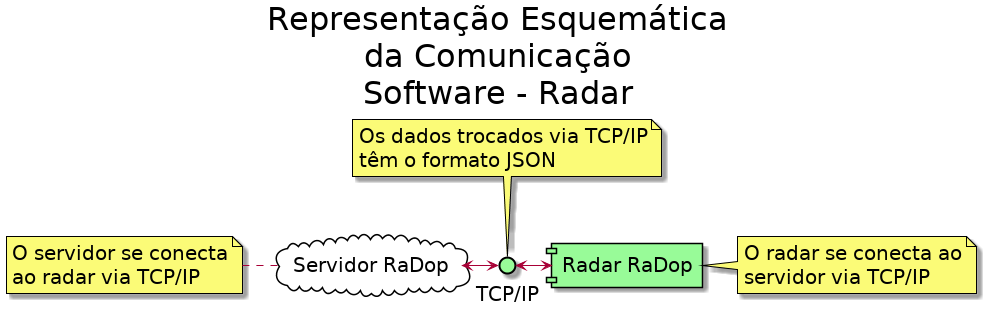
\includegraphics[width=\textwidth]{diagrama-comunicacao-software-radar.png}}
	\caption{\label{fig:diagrama-com-soft-radar} Representação de como é a comunicação entre o servidor RaDop e o radar.}
\end{figure}

A comunicação é feita entre o servidor do RaDop e o Radar via protocolo TCP/IP. Ambos têm um endereço IP pelo do qual são acessados. Esses endereços têm um único \textit{endpoint} para ser acessado nas comunicações, independente do tipo de dado enviado.

Como há um único \textit{endpoint} de ambos os lados, a diferenciação do tipo de comunicação sendo realizada é por intermédio do JSON que está no \textit{payload} da mensagem enviada. Nele, há um atributo denominado "type", e através dele é determinado do que se trata a comunicação que está sendo feita.

Por fim, para confirmar o recebimento de um pacote, o recebedor deve mandar uma resposta que atesta que o dado foi recebido.

\section{Banco de Dados}

Os produtos de software desenvolvidos pela equipe têm os seus dados divididos em dois bancos de dados, devido ao formato da construção de alguns sistemas.

Os sistemas de microsserviços trabalham de forma descentralizada e, em sua maioria, trabalham com objetos JSON. Devido a este formato de trabalho, o banco de dados escolhido foi o \textit{RethinkDB}. Ele é um banco de dados \textit{NoSQL} de chave e valor, muito parecido com a natureza descritiva do JSON. Por consequência, a aplicação RaDop -- que está fortemente apoiada nos microsserviços -- faz uso do mesmo banco de dados, mas em um domínio próprio para os próprios dados.

O sistema do \textit{Dashboard}, devido ao estilo arquitetural MVT (\textit{Model}, \textit{View} e \textit{Template}) e o mapeamento objeto-relacional (ORM, ou \textit{Object-Relational Mapping}) do \textit{Django}, a aplicação trabalha melhor com bancos de dados relacionais. Por isso, optou-se por usar um banco de dado relacional SQL, o \textit{PostgreSQL}. Ele faz parte do \textit{stack} de serviços que dão apoio ao \textit{Dashboard}.

A partir dessa escolha a equipe elaborou, com base nos requisitos e necessidades até aqui levantados, um modelo de classe que englobe os dois bancos de dados, que está melhor descrito na subseção abaixo.

\subsection{Diagrama de Classes}

A equipe de software do RaDop construiu a Figura \ref{fig:diagrama-classe-soft} para representar como é o modelo de dados/objetos das aplicações de software. Devido ao fato de que grande parte dos sistemas trabalham com tecnologias de JSON para o armazenamento de objetos, as classes derivaram destes arquivos definidos durante a execução dos sistemas.

\begin{figure}[H]
	\center{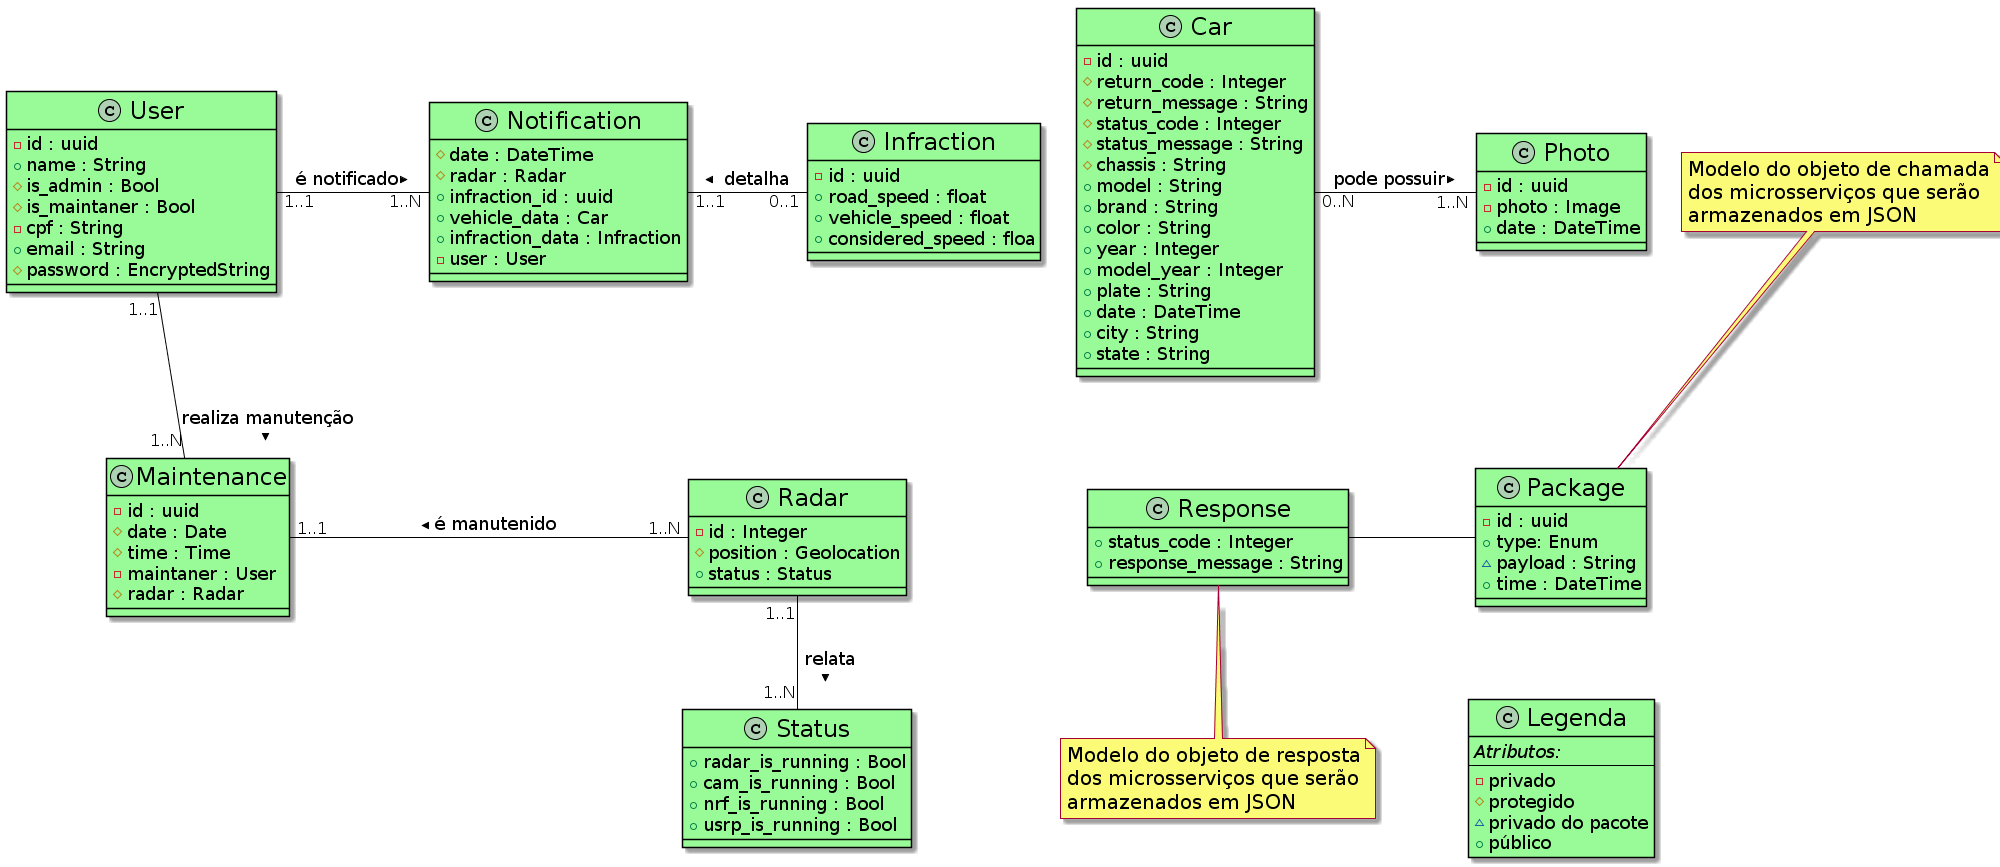
\includegraphics[scale=0.20]{classes.png}}
	\caption{\label{fig:diagrama-classe-soft} Diagrama UML de classes dos produtos de software.}
\end{figure}


O JSON é um acrônimo de \textit{JavaScript Object Notation}. É um formato compacto, de padrão simples, rápido, aberto e independente de troca de dados (\textit{parsing}) entre sistemas. Ele foi especificado por Douglas Crockford em 2000 e utiliza texto legível à humanos, no formato atributo-valor (natureza auto-descritiva)\cite{jsonorg}.

A partir disso, a equipe elaborou de uma forma simples e explicativa de como se dão as classes de objetos e suas relações por meio da representação em UML. Cabe lembrar que novas classes, relacionamentos e atributos podem ser criados na medida em que for necessário.

As classes representadas como \textit{Response} e \textit{Package} são as classes representativas dos objetos de mensagem que são trocados entre o Radar e o servidor de microsserviços, e posteriormente às aplicações.

\section{Resiliência na Comunicação do Software}

A comunicação dos diversos softwares entre si e com o radar são essenciais para o funcionamento do sistema neste projeto. Por isso, deve-se tornar o sistema criado o mais resiliente possível com relação à problemas de comunicação, para que o impacto desses seja o menor possível, caso ocorram.

Por isso, foram levantados os principais problemas possíveis de ocorrer, dentro do escopo do presente projeto, na comunicação entre os softwares ou destes com o radar. A partir disso, foi-se definido que tipo de mecanismos estão presentes para mitigar os efeitos dessas falhas para o funcionamento do sistema como um todo.

Abaixo estão listadas as falhas possíveis de ocorrerem, assim como as medidas para mitigar os efeitos delas:

\subsection{Impossibilidade de comunicação entre o radar e o sistema remoto}

\begin{itemize}
    \item \textbf{Descrição da falha:}

    A comunicação entre o radar e o sistema remoto é interrompida, impossibilitando a troca de dados entre ambos.

    \item \textbf{Mecanismo para mitigar a falha:}

    Os dados que não puderem ser enviados são armazenados localmente (no serviço remoto) e transmitidos assim que a comunicação for restabelecida. Isso faz com que dados não deixem de ser enviados em caso de falha de comunicação.
\end{itemize}

\subsection{Impossibilidade de comunicação com algum microsserviço}

\begin{itemize}
    \item \textbf{Descrição da falha:}

     O envio ou recebimento de dados de um microsserviço é impossibilitado.

    \item \textbf{Mecanismo para mitigar a falha:}

    Toda nova requisição, independente se o serviço está ou não sem comunicação, é colocada em uma fila de execução. Isso faz com que, enquanto o microsserviço não for reestabelecido, o fluxo normal não prossiga.

    Além disso, o uso da fila proporciona uma organização na ordem de execução dos pedidos. A ferramenta que é utilizada para gerenciar essas filas é o \textit{RabbitMQ}.
\end{itemize}

\subsection{Queda de um microsserviço}

\begin{itemize}
    \item \textbf{Descrição da falha:}

    Um microsserviço se torna indisponível, entendendo indisponibilidade como ele travar ou ser encerrado.

    \item \textbf{Mecanismo para mitigar a falha:}

    Os microsserviços são colocados em contêineres da tecnologia \textit{Docker}. Isso permite que novas instâncias de microsserviços indisponíveis sejam criadas rapidamente, fazendo com que o tempo de indisponibilidade deles seja reduzido.

    Além disso, o uso dos contêineres permitem que várias instâncias semelhantes de um microsserviço estejam em funcionamento ao mesmo tempo e sejam criadas ou removidas a qualquer momento. Desse modo, é possível ter uma alta disponibilidade dos microsserviços, assim como escalabilidade.
\end{itemize}

\section{\textit{DevOps}}

\textit{DevOps} é um termo criado a partir da união de dois termos, o \textit{Dev} é atribuido ao \textit{development}, ou seja, a parte de desenvolvimento da organização. Já o \textit{Ops} diz respeito à \textit{operations}, o setor da organização relacionado à operações. O \textit{DevOps} descreve um conjunto de práticas para integração entre os setores de desenvolvimento, operações, além da adoção de processos automatizados para produção rápida e segura de aplicações e serviços. É um processo que é factível o desenvolvimento ágil de aplicações.

Segundo Ebert \cite{ebert2016devops} o \textit{DevOps} trata de processos de negócios de desenvolvimento e provisionamento rápidos e flexíveis. Integra de forma eficiente o desenvolvimento, a entrega e as operações, facilitando assim uma conexão enxuta e fluida desses silos tradicionalmente separados.

Dentro do projeto RaDop, a equipe de software busca seguir algumas das melhores práticas do processo para garantir agilidade e segurança durante o desenvolvimento dos produtos. As práticas implementadas são:
\begin{itemize}
    \item Integração Contínua (CI): Para garantir a qualidade e a uniformidade de todo o código novo que entra no sistema, os produtos de softwares estão inseridos em um \textit{pipeline}, no qual passam por testes de padrão de desenvolvimento, de código, estáticos, de segurança e de construção de serviços. Com a execução exitosa de todos os testes nos novos serviços, assim como nas evoluções dos antigos, eles são integrados com as versões anteriores e os demais serviços.
    \item Entrega Contínua (CD): Com a garantia de que as novas versões e evoluções estão de acordo com o planejado, esses novos produtos, ou subprodutos, são entregues e implementados no destino (serviço do servidor, aplicativo ou \textit{Dashboard}) mais rapidamente e estam prontamente disponíveis para uso.
    \item \textit{Docker}: Para provisionamento dos serviços, implantação e isolamento dos ambientes e requerimentos. Também auxilia na escalabilidade dos serviços e possibilitar ações ágeis sobre erros e dificuldades.
\end{itemize}

\section{Identidade Visual}

Na construção do Dashboard e do Aplicativo foi visto a necessidade de uma identidade visual para o projeto. 

Os ícones foram feitos nos tamanhos: 512x512, 256x256, 128x128, 64x64 e 32x32.

A figura \ref{fig:identidade_visual}, apresenta os ícones usados no aplicativo e no dashboard.

\begin{figure}[H]
	\center{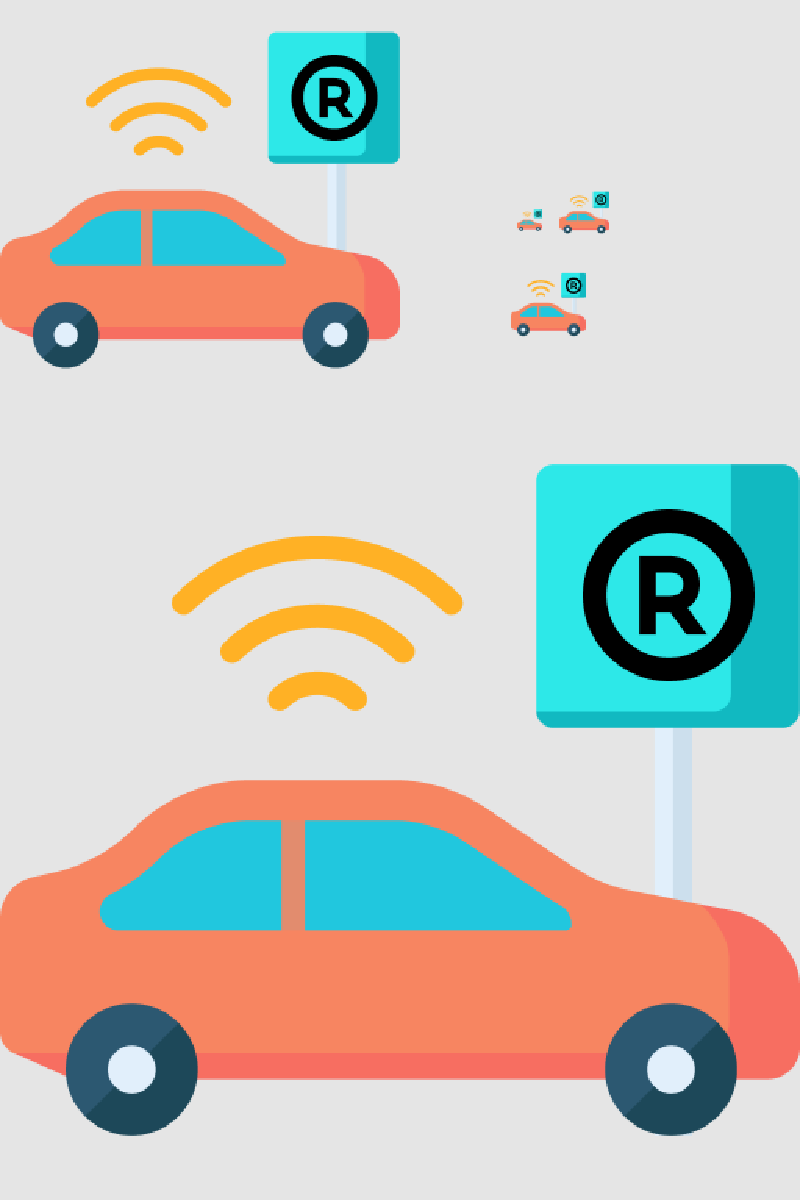
\includegraphics[scale=0.5]{identidade_visual.pdf}}
	\caption{\label{fig:identidade_visual} Ícones do aplicativo do radar e do dashboard nos tamanhos mencionados acima.}
\end{figure}

\section{Protótipos}

Todas as telas referentes à construção da interface entre o sistema e o usuário foram desenhadas para auxiliar o time na construção do software e pensando também na melhor usabilidade para o usuário.

A Figura \ref{fig:tela_inicial}, apresenta o protótipo da tela inicial do aplicativo RaDop.

\begin{figure}[H]
	\center{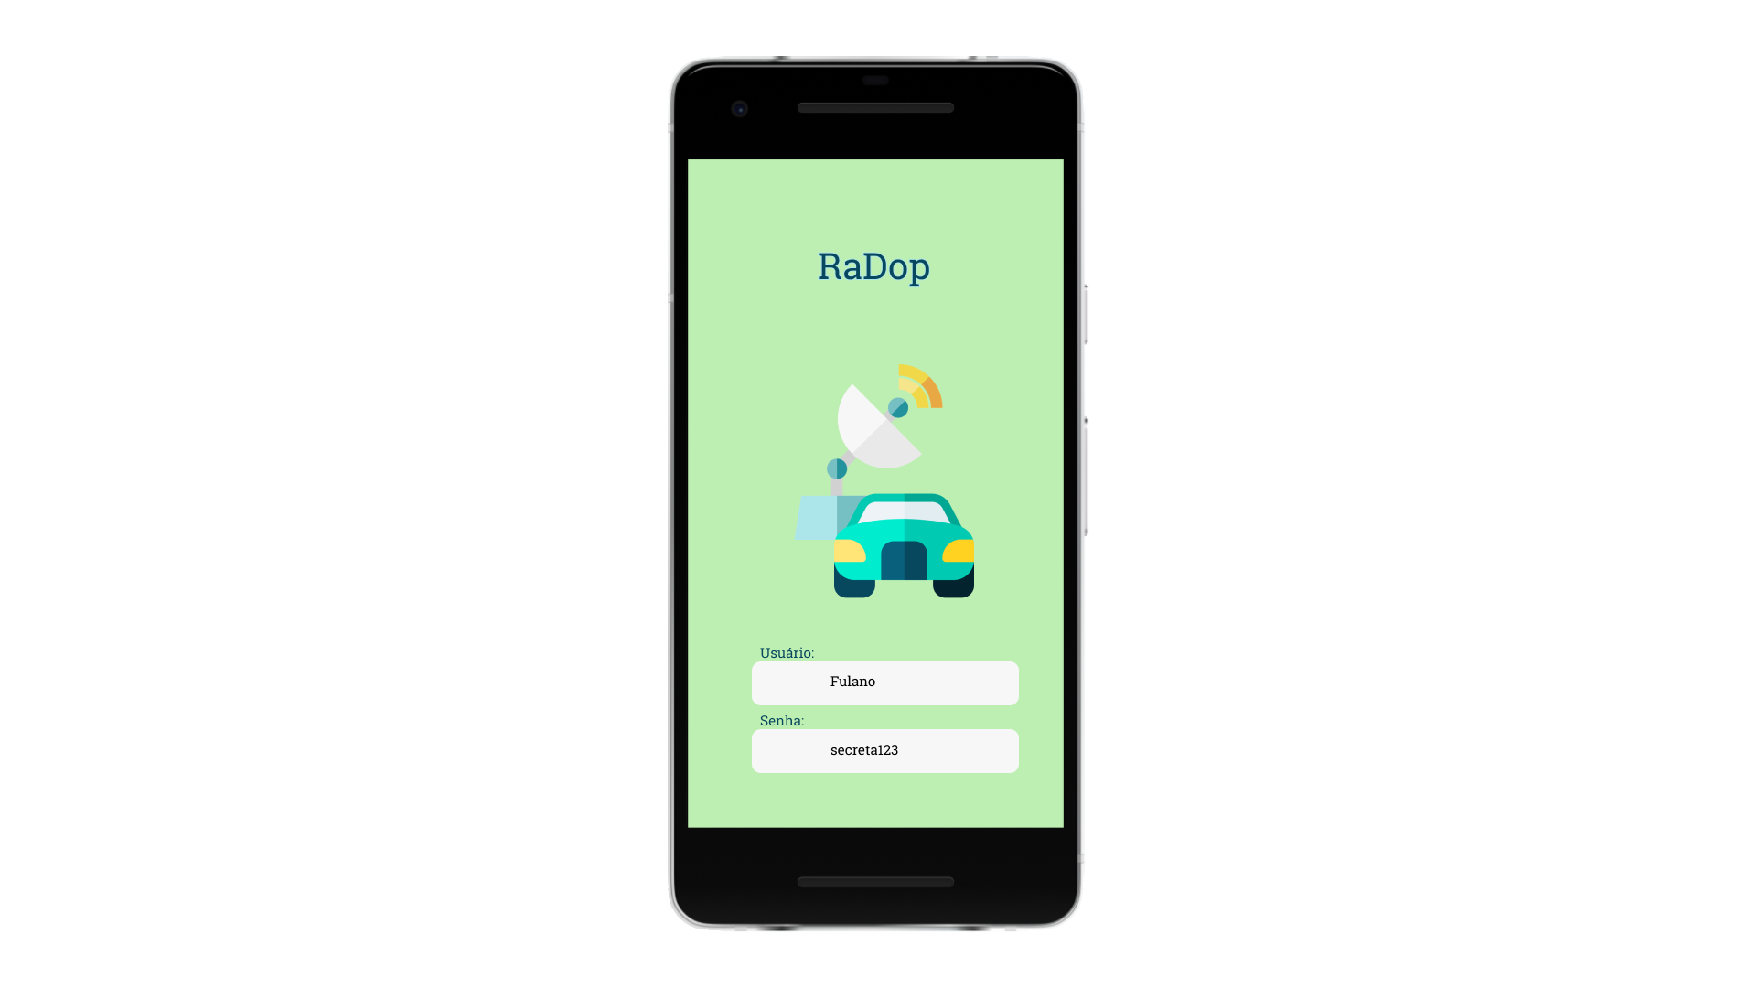
\includegraphics[scale=0.5]{tela_inicial_aplicativo.pdf}}
	\caption{\label{fig:tela_inicial} Protótipo da tela inicial do aplicativo RaDop.}
\end{figure}

A Figura \ref{fig:tela_status}, apresenta o protótipo da tela com os estados de funcionamento do radar.

\begin{figure}[H]
	\center{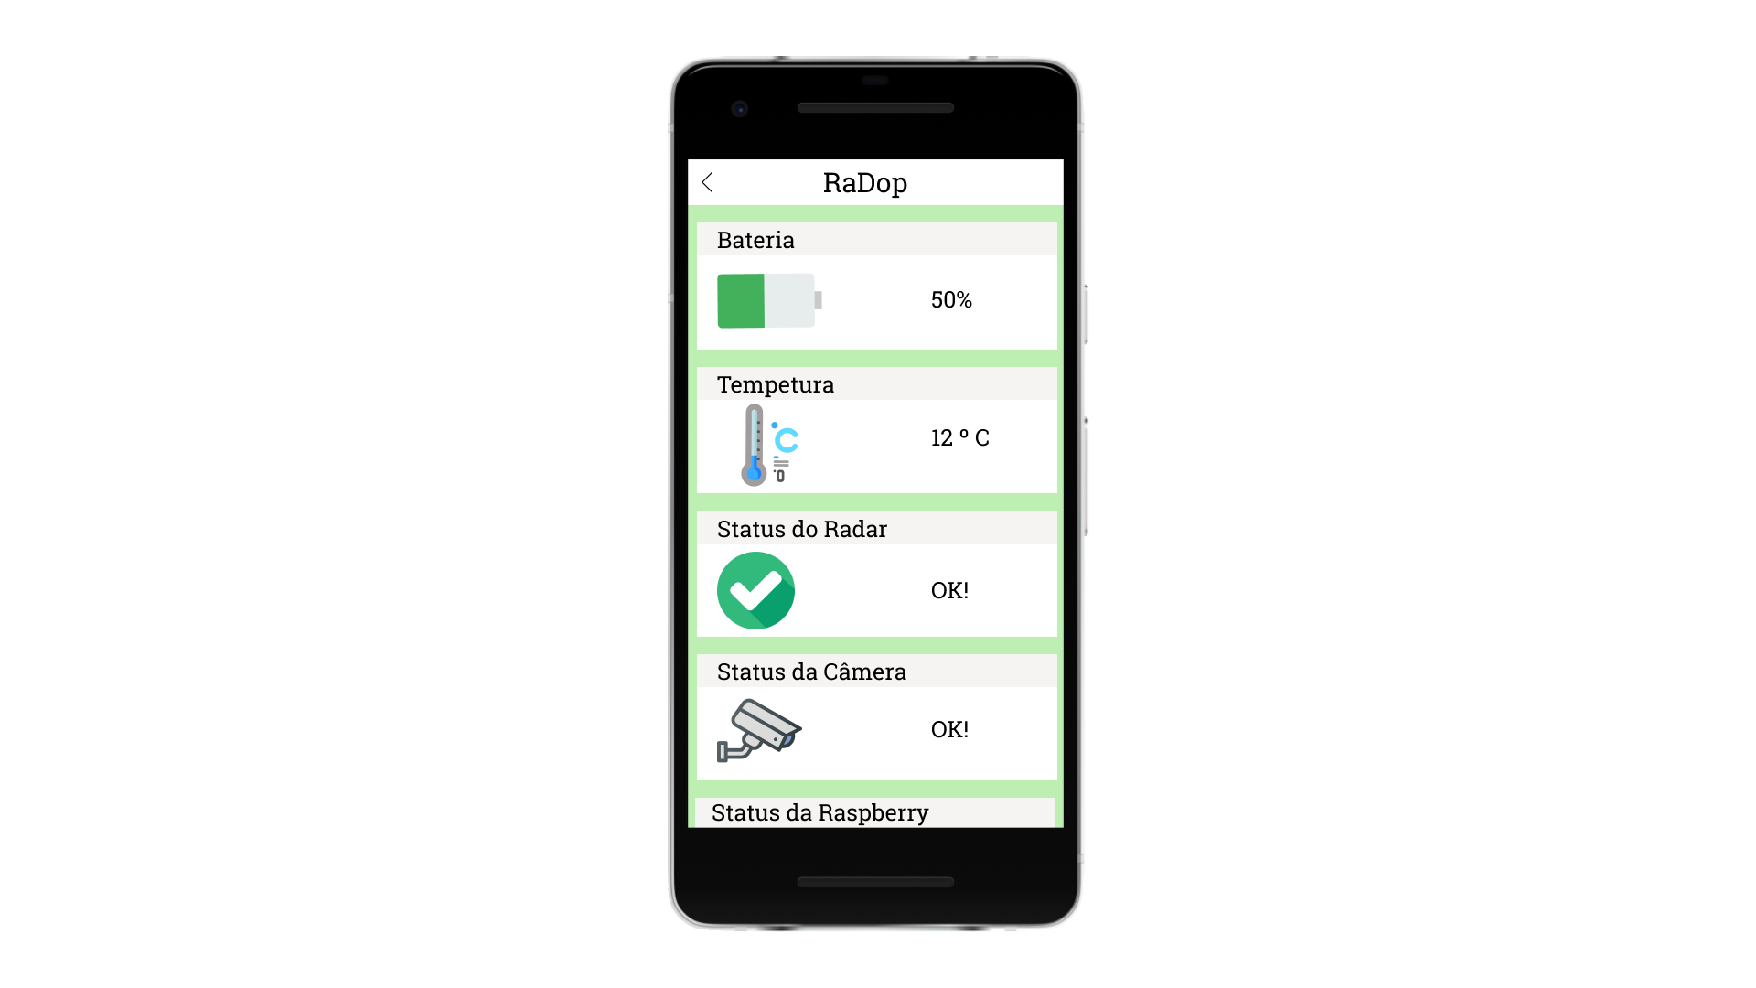
\includegraphics[scale=0.42]{tela_status.pdf}}
	\caption{\label{fig:tela_status} Protótipo da tela com os estados de funcionamento do radar.}
\end{figure}

A Figura \ref{fig:tela_registro}, apresenta o protótipo da tela de registro para o usuário administrador poder cadastrar a manutenção do radar.

\begin{figure}[H]
	\center{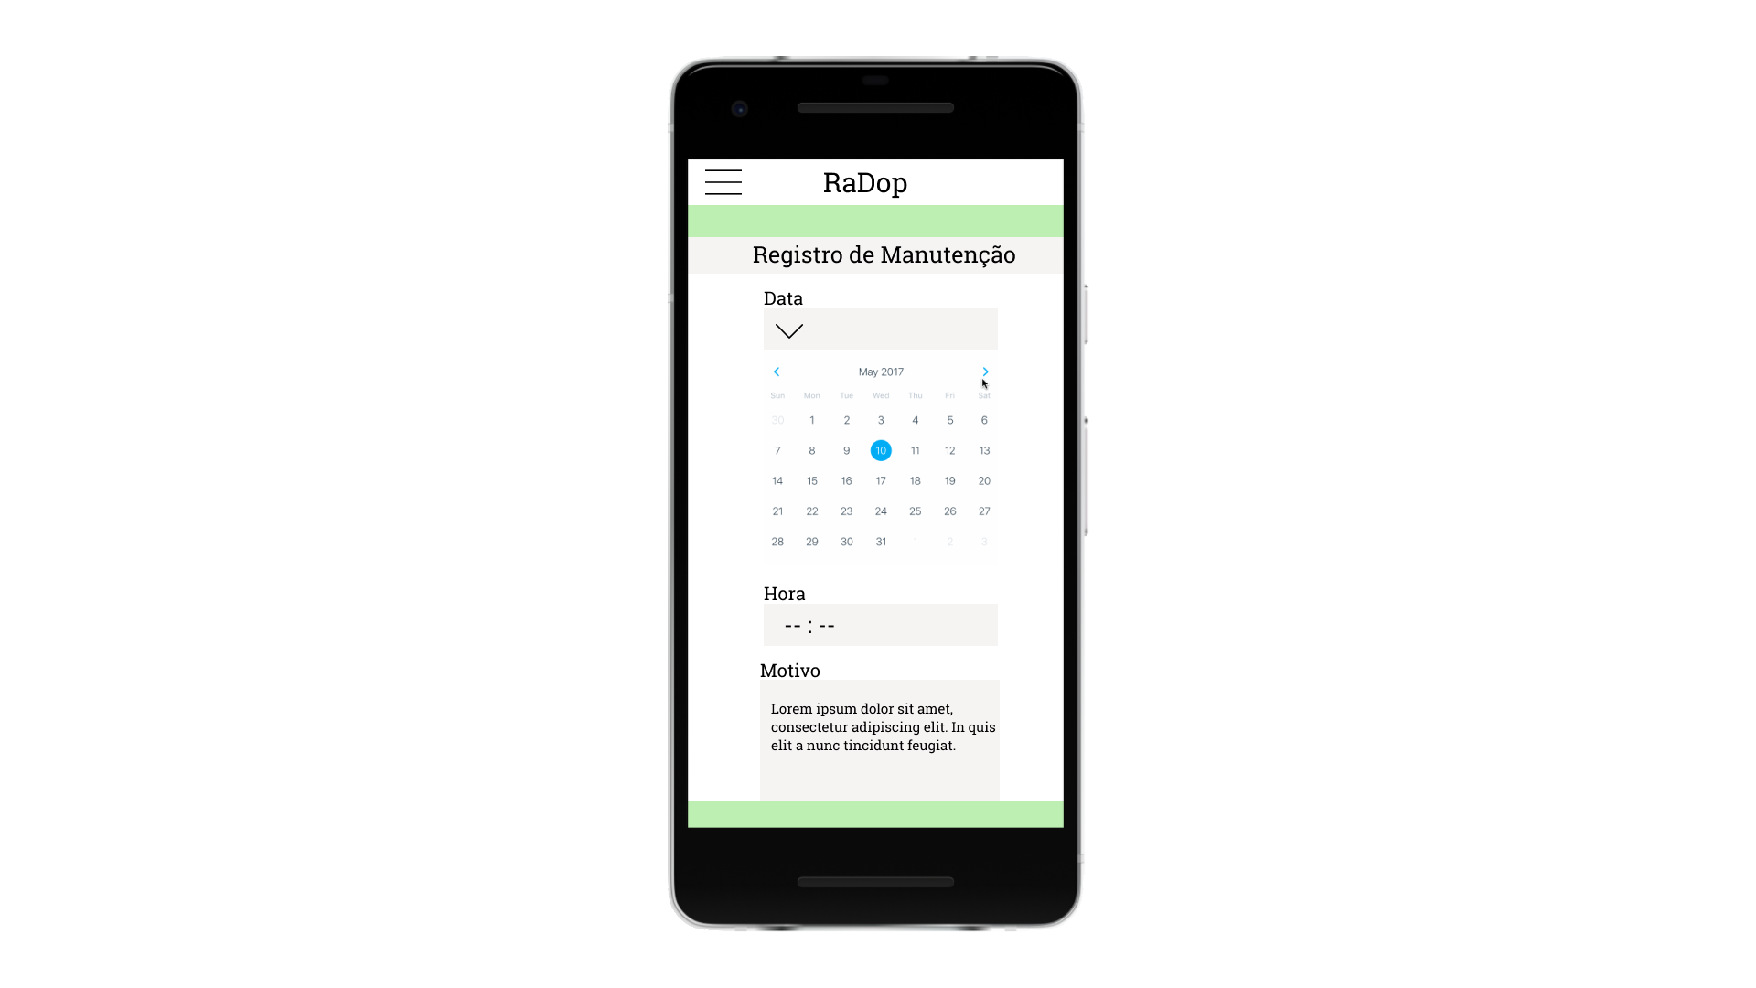
\includegraphics[scale=0.42]{tela_registro.pdf}}
	\caption{\label{fig:tela_registro} Protótipo da tela de registro para o usuário administrador poder cadastrar a manutenção do radar.}
\end{figure}

A Figura \ref{fig:tela_dashboard}, apresenta o protótipo da tela principal do dashboard do radar.

\begin{figure}[H]
	\center{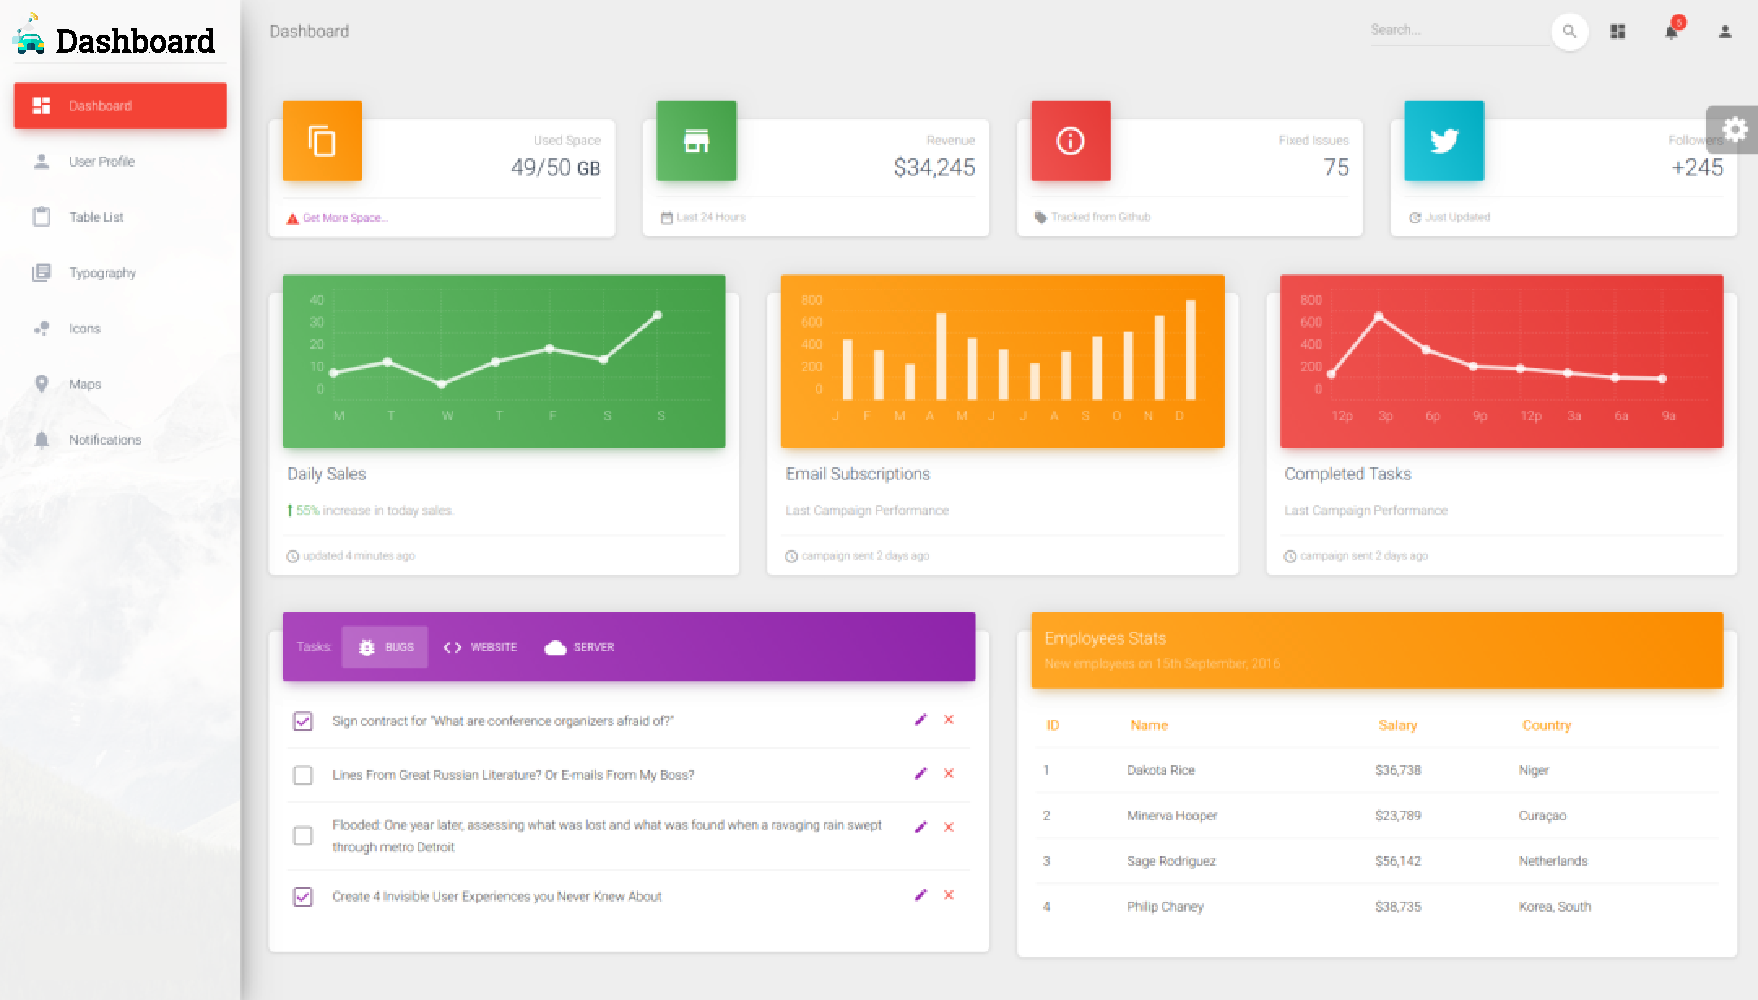
\includegraphics[scale=0.5]{tela_dashboard.pdf}}
	\caption{\label{fig:tela_dashboard} Protótipo da tela principal do dashboard do radar.}
\end{figure}

\pagebreak
